%! Author = jaroslavtoth
%! Date = 29/12/2023

% Preamble
\documentclass[11pt]{article}

% Packages
\usepackage{amsmath}
\usepackage{graphicx}
\usepackage[numbers]{natbib}

\graphicspath{{figures/}}
\title{Designing Internal Synchronous Software API}
\author{Jaroslav Tóth \\\textit{xtothj@gmail.com}}
\date{\today}

% Document
\begin{document}
\maketitle

\section{Introduction}
\label{sec:introduction}
Modeling a software API (Application Programming Interface) is an essential part of the software design
and development process.
Making poor decisions during the design phase can lead to numerous issues in the future, including increased
maintenance costs, decreased flexibility of the API, and hindering the evolution of the next API\@.
These issues are further compounded by the fact that the API is utilized by other components in the system.

This guide focuses on the most commonly used design patterns and approaches that can be leveraged during
the creation or refactoring of internal synchronous software APIs. Each approach has its own benefits
and drawbacks and should be employed in the right context.
When we refer to an internal API, we mean an API that is used by other components in the same process between
different software components, such as modules or classes, typically described by specific interfaces.
However, some of the described patterns can also be applied to model external or asynchronous interfaces.

The guide emphasizes the structure of the API more than how components communicate with each other.
Additionally, the document does not delve into the implementation details of the API,
such as specific technologies or languages, but rather focuses on general design principles.

The paper is structured as follows.
The first part describes the requirements and analysis of the target domain, which will be used as an example.
The subsequent sections detail design approaches and related design patterns,
demonstrated on the example using UML diagrams.
This starts with the Singleton Interface Method approach, progresses through object-oriented approaches,
and concludes with the Model-Driven API\@.
The final part provides a summary of the content, presenting a metamodel view of all the approaches.


\section{Requirements}
\label{sec:requirements}
Let's assume that we are designing API for sending of the Internet Group Management Protocol version 2 (IGMPv2)
packets over the network.
There are following simple requirements that should be fulfilled by the designed and implemented service API:

\begin{itemize}
    \item Service must be able to serialize IGMPv2 packets into the output buffer.
    \item Service must be able to serialize all types of IGMPv2 packets - Membership Query, Membership Report,
    and Leave Group message.
    \item Parameters of the IGMPv2 packet should be configurable by the client using human-readable values.
    \item If client does not specify any value for the parameter, default values should be used.
\end{itemize}


\section{Domain Analysis}
\label{sec:domain}
The first step in the design process is to understand the domain of the API. It helps to identify required
input parameters, return values, and types expressed in the domain language.
It is also important to capture possible API evolution in the future, so the modeled API is flexible enough
to support it without drastic changes and breaking backwards compatibility.

There are 3 types of the IGMPv2 messages - Membership Query, Membership Report, and Leave Group message.
All types of messages follow the same format of the packet header but with different values in the fields.
The structure of the IGMPv2 packet is depicted in the Figure~\ref{fig:igmp_packet}.

\begin{figure}[!htb]
\centering
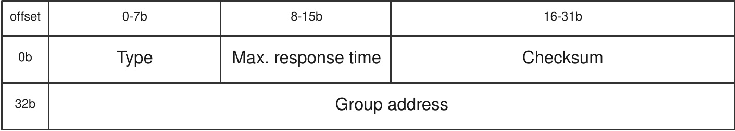
\includegraphics[width=1.0
\textwidth]{igmp_packet}
\caption{Structure of the IGMPv2 packet}
\label{fig:igmp_packet}
\end{figure}

From the perspective of the API design, there are following key differences between constructed types of packets:

\begin{enumerate}
    \item Membership Query - Type field is set to 0x11 value.
    Both maximum response time and group address can have non-zero value.
    In case of General Query, group address is set to \textit{0.0.0.0} value (all multicast groups are queries
    in the broadcast domain).
    In case of Group-Specific Query, group address should contain valid multicast address that is queried by router.
    \item Membership Report - Type field is set to 0x12 value.
    Maximum response time is always set to 0 (unused).
    Group address should contain valid multicast address reported by client.
    \item Leave Group - Type field is set to 0x17 value.
    Maximum response time is always set to 0 (unused).
    Group address should contain valid multicast address that client wants to leave.
\end{enumerate}

The following list summarizes the findings from the domain analysis which we have to keep in mind during
the design process:

\begin{itemize}
    \item There are 3 types of the IGMPv2 messages that differ in the constant values of the fields.
    Serialization logic, that will be implemented as the business logic, is common for all types of messages.
    \item There are 2 configurable parameters (aside from the type of message) that client should be able to specify
    on the input - maximum response time and group address.
    However, there are some constraints on the values of these parameters based on the type
    of the IGMPv2 message (for example, Leave Group message maximum response time is always set to 0)
    and field length (number of bytes).
    \item API should not contain any return type since serialized data will be written to the output stream
    (for example, backed by network socket) that is passed as the input parameter.
    \item In the future client may require to support also IGMPv1 and IGMPv3 protocols.
    Especially IGMPv3 protocol specify additional fields in the packet header that are not present
    in the IGMPv2 protocol.
    There is also open room for possible support of IPv6 flavour of the IGMP protocol
    - Multicast Listener Discovery (MLD) that is implemented by the Internet Group Management Protocol (IGMP).
\end{itemize}


\section{Singleton Interface Method}
\label{sec:singleton_interface_method}
Singleton Interface method is based on fitting of all the parameters and customizations into single method definition.
Usually some of the parameters are nullable because there is some default value that is used in case
of the null value (specified in the business logic) or the parameter is not used at all in combination
with other parameters (for example, maximum response time is not used in case of the Leave Group message).
It is the simplest approach that can be used for designing of the API\@.

The Figure~\ref{fig:sing_write_igmp_packet} shows the activity diagram with interface definition of the
method for writing of the IGMPv2 packet into the output stream.
All parameters including type of the message are squashed into the single interface method.
Only parameters \textit{igmpType} and \textit{outputStream} are mandatory, other parameters may contain null values
depending on the value of \textit{igmpType} parameter.

\begin{figure}[!htb]
    \centering
    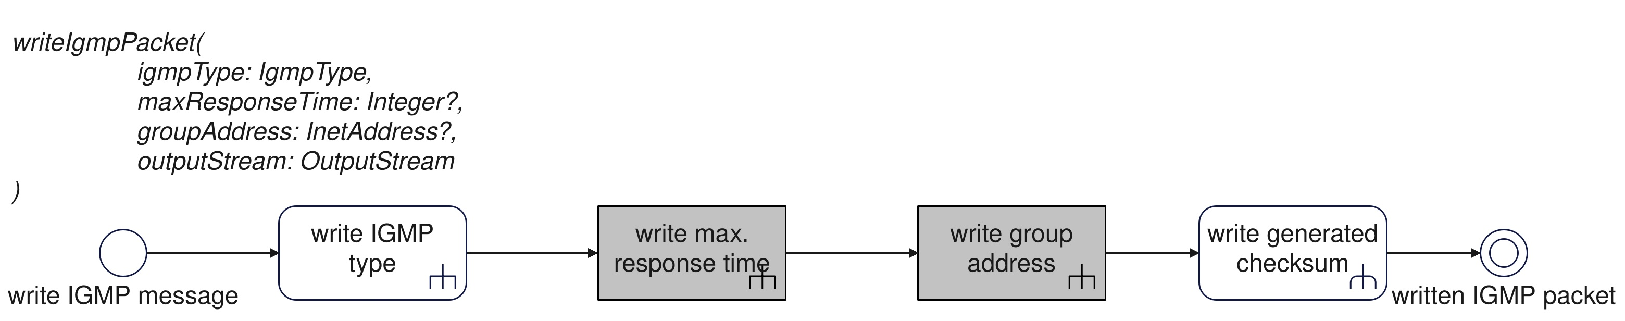
\includegraphics[width=1.0
    \textwidth]{sing_write_igmp_packet}
    \caption{Singleton Interface Method: Writing IGMP packet using }
    \label{fig:sing_write_igmp_packet}
\end{figure}

Activity diagram also contains more complex activities (write maximum response time and write group address)
that must be decomposed into the smaller diagrams.
For example, content of the write maximum response time activity is depicted
in the Figure~\ref{fig:sing_write_max_response_time}.
Since the whole logic is implemented under common interface method, the business logic contains a lot of branching
including conditional statements that are used for handling invalid combinations of the input parameters.

\begin{figure}[!htb]
    \centering
    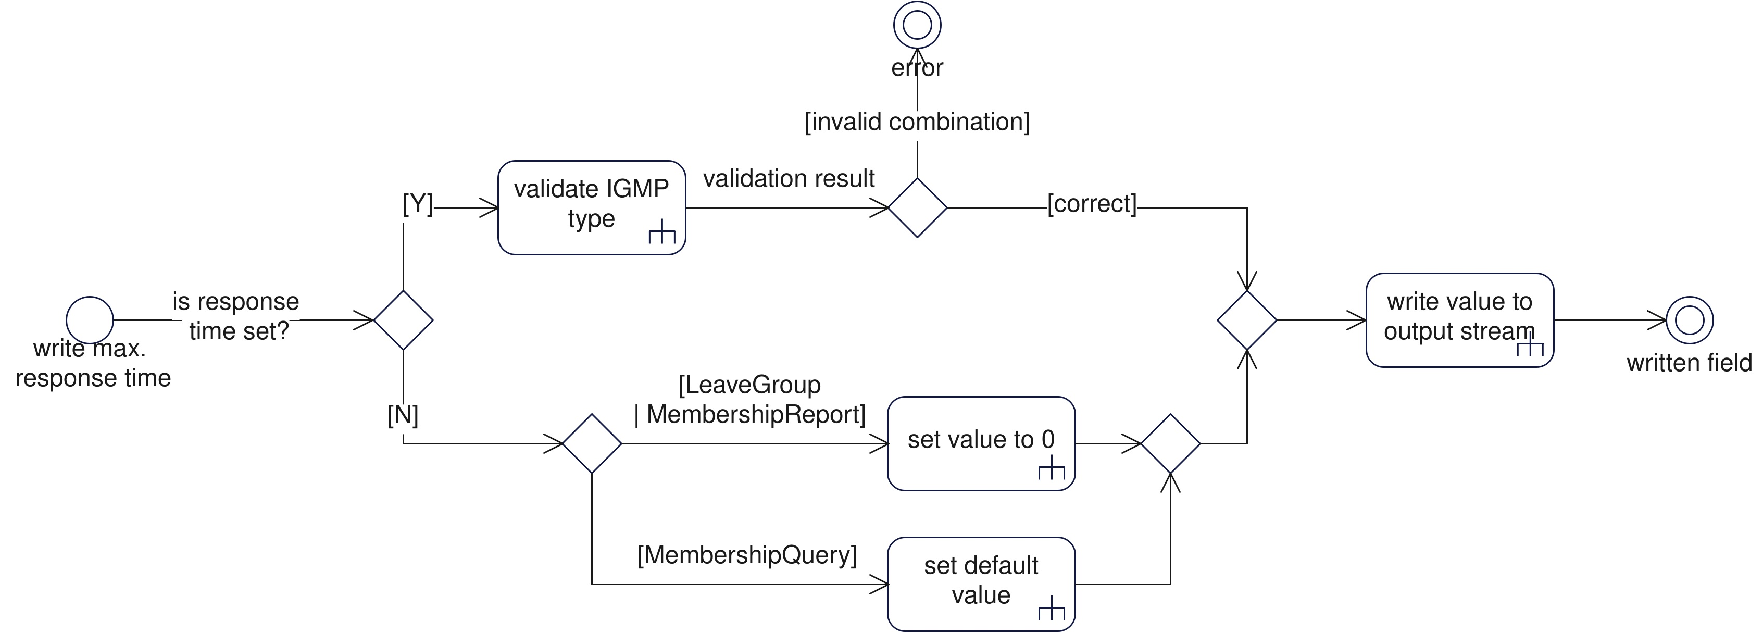
\includegraphics[width=1.0
    \textwidth]{sing_write_max_response_time}
    \caption{Singleton Interface Method: Writing maximum response time}
    \label{fig:sing_write_max_response_time}
\end{figure}

Benefits of the Singleton Interface Method:

\begin{itemize}
    \item Implementation of the interface is straightforward and simple.
    There is no need to implement any additional software entities.
    \item Single point of the contact for the API client may be beneficial in some cases.
    For example, client may represent just some additional proxy layer on top of the API that
    already receives all the required parameters from the other components in the system.
    Further decomposition of the layer would introduce unnecessary complexity in the proxy layer
    (calling correct method exposed by service based on some conditions).
\end{itemize}

Drawbacks of the Singleton Interface Method:

\begin{itemize}
    \item Appearance of God Classes/Functions - All the logic is implemented in single method which is usually
    very complex with a lot of branching.
    It is usually difficult to understand the logic and maintain it in the future.
    \item Evolution of the API is very hard - Supporting next packet fields, for example in case of the IGMPv3,
    would require to change the interface method signature and all the clients that are using it.
    \item Nullable parameters - Some of the parameters are nullable depending on the type of the IGMP message.
    Implementation must contain additional logic for handling of the invalid combinations of the parameters
    and client must be aware of the valid combinations.
    Additionally, default values that override null values are not transparent to client and must be explicitly
    documented.
    \item Long list of parameters is error-prone.
    If used technology does not support named parameters, client must be aware of the ordering.
    \item Violation of the Single Responsibility Principle (SRP) - Such methods tends to grow over time
    and usually contain more than one responsibility.
\end{itemize}

Common use-cases of the Singleton Interface Method:

\begin{itemize}
    \item Stable API that is not expected to change in the future,
    and it does not contain complex branching in the implementation.
    There is just single behaviour that is implemented by the service without customizations or subtypes.
    \item Simple services or utility functions with small number of non-null parameters.
\end{itemize}


\section{Method Multiplication}
\label{sec:method_multiplication}
The Method Multiplication approach involves decomposing the API into multiple interface methods,
with decomposition based on responsibility, functionality, parameter types, or the nullability of certain parameters.
This decomposition is a delicate balance between usability and API complexity; the functionality should not be overly
fine-grained or excessively spanned across multiple interface methods.

Figure~\ref{fig:mult_decomposition_by_type} illustrates the decomposition of the API based on IGMPv2 types.
The previous version of API (Figure~\ref{fig:sing_write_max_response_time}) is split into three interface methods,
each dedicated to a specific message type
\footnote{
    The subsequent diagrams exclude the calculation of the checksum, as it is irrelevant for illustrating API design.
    This omission remains consistent across every version of the example.
}.
This separation allows the removal of the \textit{igmpType} parameter from the interface method,
simplifying the input parameter checks in the implementation logic.

\begin{figure}[!htb]
    \centering
    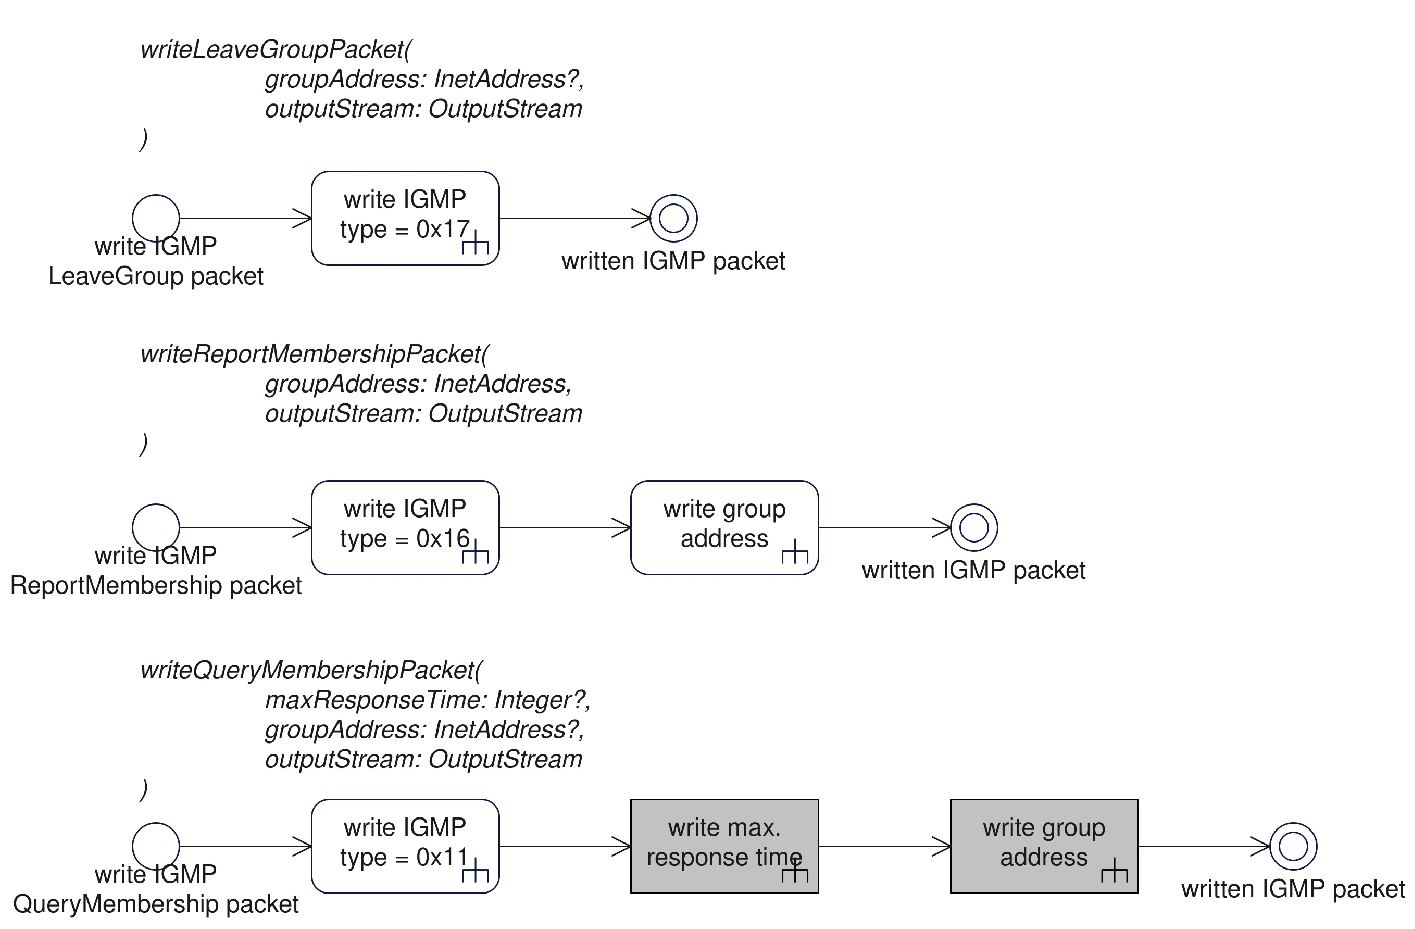
\includegraphics[width=1.0
    \textwidth]{mult_decomposition_by_type}
    \caption{Method Multiplication: Decomposition of API by type}
    \label{fig:mult_decomposition_by_type}
\end{figure}

In Figure~\ref{fig:mult_decomposition_by_type}, the writing of the IGMP Query Membership message remains complex due
to two optional parameters: \textit{maxResponseTime} and \textit{groupAddress}.
The \textit{groupAddress} is only \textit{0.0.0.0} in the case of the General Query message; otherwise,
it is a mandatory parameter.
To address this, it is sensible to split the interface method into two: one for the General Query message and another
for the Group-Specific Query message.
This decomposition is depicted in Figure~\ref{fig:mult_decomposition_by_function}.

\begin{figure}[!htb]
    \centering
    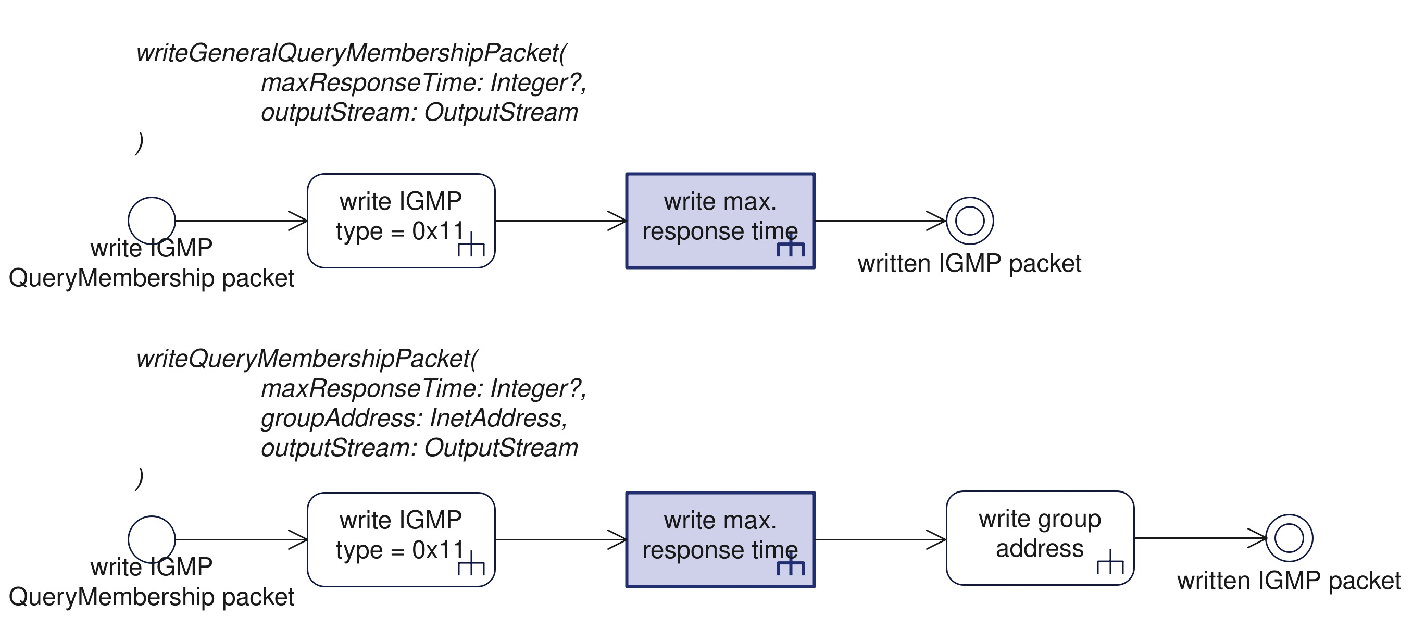
\includegraphics[width=1.0
    \textwidth]{mult_decomposition_by_function}
    \caption{Method Multiplication: Decomposition of API by functionality}
    \label{fig:mult_decomposition_by_function}
\end{figure}

Finally, Figure~\ref{fig:mult_decomposition_by_default_values} illustrates the split of the method for writing
the QueryMembership message into two overloaded interface methods - one with the \textit{maxResponseTime} parameter
and another without it, which internally sets a default value.
It is important to note that method overloading is not universally possible in all programming languages.
Moreover, it should be avoided if the methods have different functionalities.
In such cases, using different identifiers for the methods enhances readability.

\begin{figure}[!htb]
    \centering
    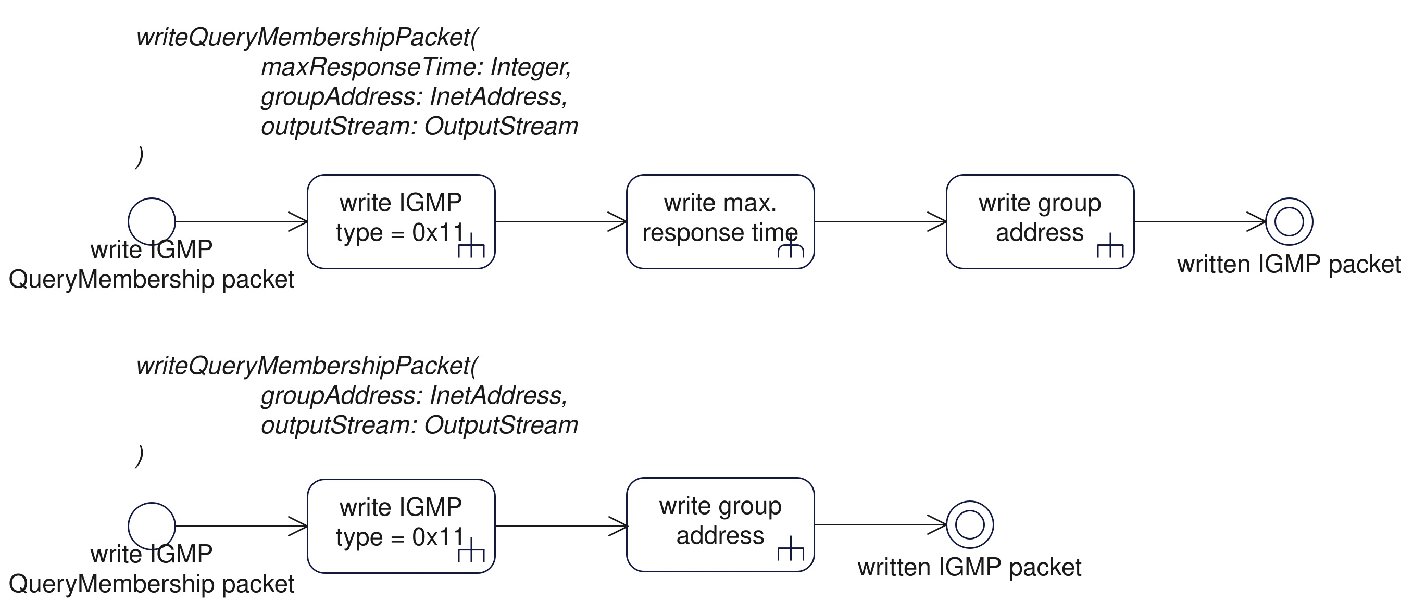
\includegraphics[width=1.0
    \textwidth]{mult_decomposition_by_default_values}
    \caption{Method Multiplication: Decomposition of API by default values}
    \label{fig:mult_decomposition_by_default_values}
\end{figure}

Other strategies for decomposition of methods include Replace Parameter with Explicit Methods or
Separate Query from Modifier refactoring patterns.
They are described in detail in the Refactoring: Improving the Design of Existing Code
book~\cite[Chapter~10]{fowler1999refactoring}.

Benefits of the Method Multiplication:

\begin{itemize}
    \item Enhanced readability and understandability:
    The API becomes more readable and understandable compared to the Singleton Interface Method.
    Well-chosen identifiers for interface methods make it easy to comprehend the purpose of the API method,
    often rendering the code self-documented.
    \item Improved maintainability:
    API maintainability is enhanced as updating or adding new functionality becomes easier.
    Changes are localized to the single interface method, simplifying the overall maintenance process.
    \item Enhanced robustness:
    The API becomes more robust as it prevents the invocation of methods with invalid parameter combinations.
    \item Mitigation of God Methods:
    The implementation of the API is distributed across multiple methods, addressing the issue of God Methods.
\end{itemize}

Drawbacks of the Method Multiplication:

\begin{itemize}
    \item Potential for God Classes:
    While the API is decomposed, there may still be a single service implemented by a class, leading to potential
    growth over time.
    Consideration of further division into multiple services, especially through Vertical Slicing, may be beneficial.
    \item Client decision overhead:
    Clients must decide which method to call, often necessitating the implementation and maintenance of another
    Facade layer on top of the API to hide the complexity around correct interface method calls.
    Read more about the Facade design pattern in the book Pattern-Oriented Software Architecture, Volume 4:
    A Pattern Language for Distributed Computing ~\cite[Chapter~12]{posa4}.
    \item Risk of Spaghetti Code in God Classes:
    The presence of God Classes may lead to Spaghetti Code, characterized by a lack of structure and organization.
    This can result from rushed or unplanned coding, leading to a complex and tangled control structure.
    Figure~\ref{fig:mult_spaghetti_code} shows an example of the Spaghetti Code in the early stage.
    There are multiple shared procedures that are called by API methods with unclear control flow.
    Internal functions tend to contain a lot of parameters that are passed between them.
    \footnote{
        The term Spaghetti Code is often attributed to computer scientist Edsger Dijkstra.
        He used it in his 1972 Turing Award lecture titled The Humble Programmer~\cite{dijkstra1972humble}.
    }
    \item API Rooting:
    Implementations of interface methods might simply call another common method, potentially internal or represented
    by another public interface method
    This implies that while the API is decomposed, the internal implementation remains
    in the Singleton Interface Method.
    Figure~\ref{fig:mult_api_rooting} provides an example of API Rooting.
\end{itemize}

\begin{figure}[!htb]
    \centering
    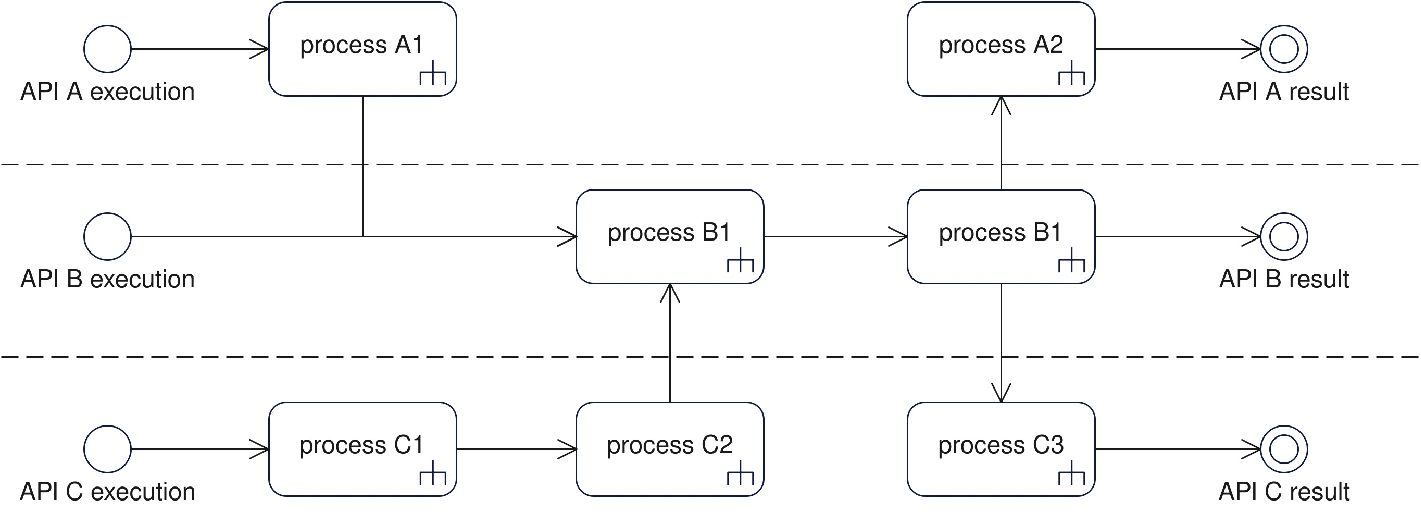
\includegraphics[width=1.0
    \textwidth]{mult_spaghetti_code}
    \caption{Method Multiplication: Germ of the Spaghetti Code}
    \label{fig:mult_spaghetti_code}
\end{figure}

\begin{figure}[!htb]
    \centering
    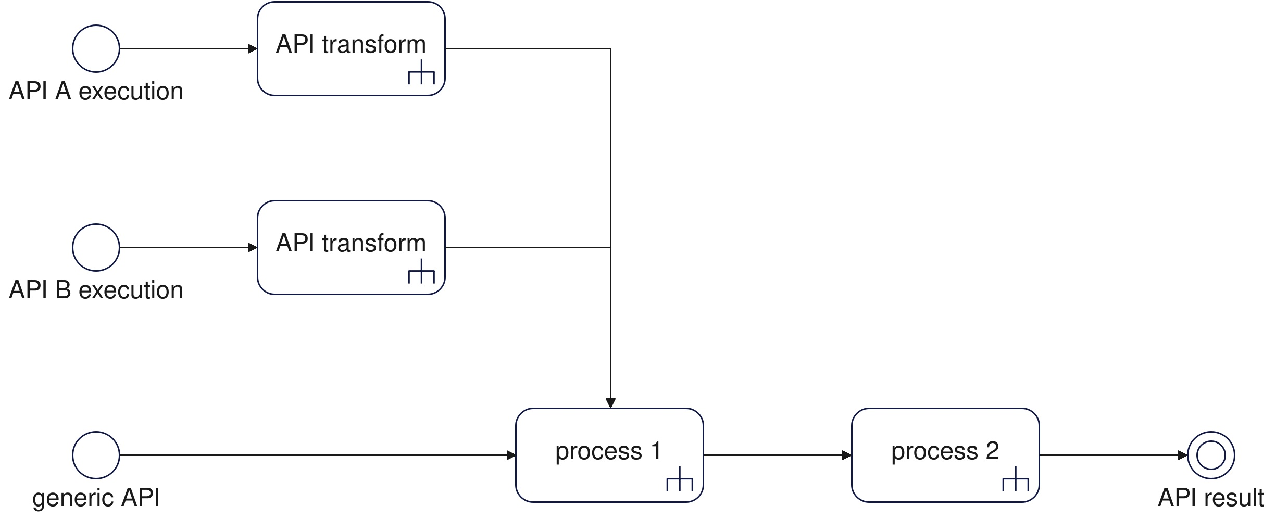
\includegraphics[width=1.0
    \textwidth]{mult_api_rooting}
    \caption{Method Multiplication: API Rooting}
    \label{fig:mult_api_rooting}
\end{figure}

Common use-cases of the Method Multiplication:

\begin{itemize}
    \item Decomposition by functionality:
    Decomposing the API by functionality into multiple interface methods is a common use-case for Method Multiplication.
    \item Overloading for parameter types:
    Overloading interface methods is utilized to support different types of input parameters.
\end{itemize}


\section{Batch Method}
\label{sec:batch_method}
The Batch Method is a design pattern enabling users to invoke a method on a collection of objects.
Usually, the method implementation is optimized to process the collection of objects in more efficient way
than executing the same operation individually in a loop on the client side.
Typically, it involves pairs of methods - one operating on a single object and another on a collection of objects.
This design pattern can be seen as a specific subtype of the Method Multiplication approach.
The book Pattern-Oriented Software Architecture, Volume 4 describes this design pattern
in detail~\cite[Chapter~12]{posa4}.

In Figure~\ref{fig:batch_write_packets}, the application of the Batch Method design pattern to the API method
for writing a collection of IGMP Query Membership packets is depicted.
Several adjustments are made compared to the single-packet method:

\begin{itemize}
    \item
    The method is named \textit{writeQueryMembershipPackets} to better reflect its functionality.
    \item
    The method now accepts a collection of group addresses queried by the IGMP Query Membership packets.
    \item
    Instead of a single \textit{OutputStream} stream bound to a single network interface, the method now accepts
    a collection of \textit{NetInterface} objects.
    The intention is to capitalize on the Batch Method design pattern's advantages and distribute the workload among
    multiple output network interfaces.
\end{itemize}

\begin{figure}[!htb]
    \centering
    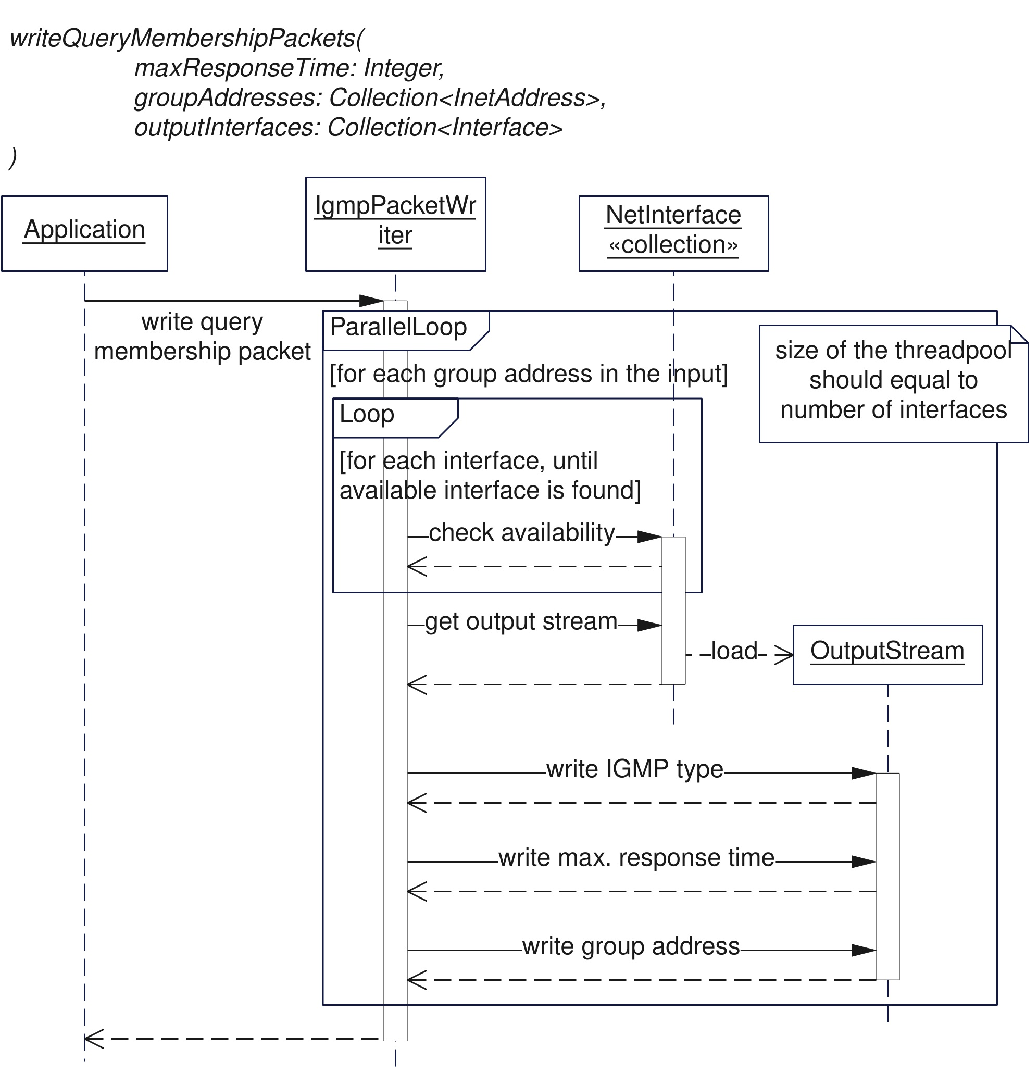
\includegraphics[width=1.0
    \textwidth]{batch_write_packets}
    \caption{Batch Method: Writing collection of IGMP Query Membership packets}
    \label{fig:batch_write_packets}
\end{figure}

Benefits of the Batch Method design pattern:

\begin{itemize}
    \item Efficiency:
    The implementation can optimize work by processing the collection of objects in a single pass,
    potentially using a single transaction and lock acquisition for multiple objects.
    Additionally, parallel processing of multiple objects may be feasible.
    \item Simplicity:
    From the client's perspective, the Batch Method design pattern is simpler to use than executing the same operation
    individually in a loop on the client side.
\end{itemize}

Drawbacks of the Batch Method design pattern:

\begin{itemize}
    \item Lack of flexibility:
    Different clients may have diverse requirements for the Batch Method.
    For instance, one client may demand atomicity, while another may not.
    It is often challenging to address all requirements with a single version of the Batch Method,
    leading to code duplication and reduced code maintainability.
    \item Artificial creation of useless Batch Methods:
    There might be a temptation to create a Batch Method for each method operating on a single object.
    However, this practice is discouraged due to increased maintenance costs, higher code complexity,
    and the likelihood of missing use-cases.
    The Batch Method design pattern should be employed only when there is a genuine use-case and when
    it can be implemented more efficiently than simple looping over the collection of objects.
\end{itemize}

Common use-cases of the Batch Method design pattern:

\begin{itemize}
    \item
    Processing multiple objects in a single transaction to ensure Atomicity, Consistency, Isolation,
    and Durability (ACID) properties.
    \item Parallel processing of multiple objects.
\end{itemize}


\section{Default Values}
\label{sec:default_values}
Some programming languages allow specification of default values directly in the method signature.
In this case, if the caller does not specify the value of the parameter, the default value is used.
This feature is often combined with named parameters.
Another approach is to specify optional parameters at the end of the parameter list.

Figure~\ref{fig:def_specification_of_default_values} shows example with specified default values in the interface
method signature.
For demonstration purposes, 2 new parameters have been added: \textit{packetLogger} used for logging serialized
packets and \textit{addressResolver} used for resolution of named addresses into IP address representation.
In this example, default values are assigned to the \textit{maxResponseTime}, \textit{packetLogger},
and \textit{addressResolver} parameters.

\begin{figure}[!htb]
    \centering
    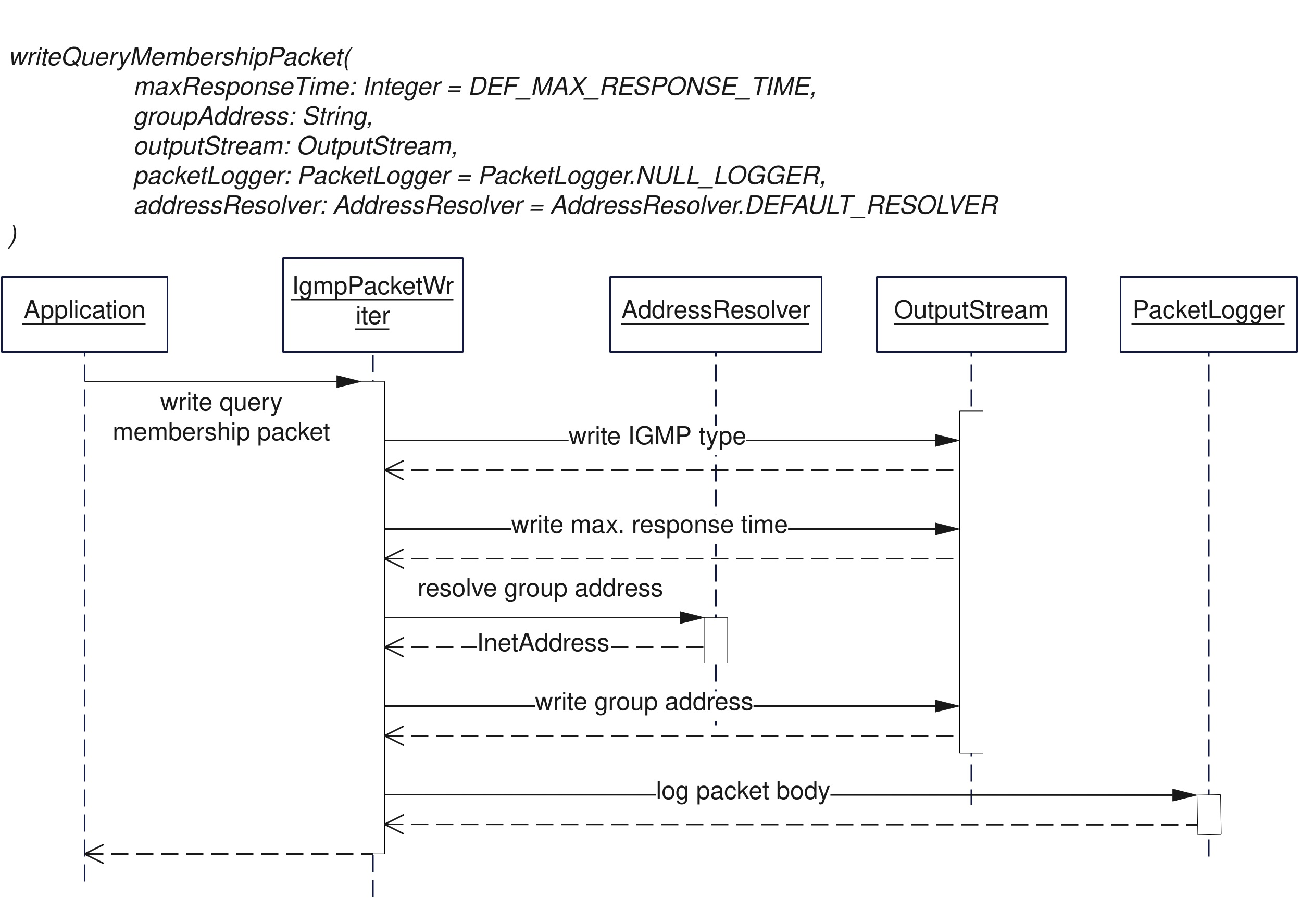
\includegraphics[width=1.0
    \textwidth]{def_specification_of_default_values}
    \caption{Default Values: Specification of default values}
    \label{fig:def_specification_of_default_values}
\end{figure}

\begin{itemize}
    \item \textit{maxResponseTime}: It has a primitive \textit{Integer} type.
    In this case, it is possible to directly specify the default value without creation of additional entities.
    \item \textit{packetLogger}: This parameter has PacketLogger type which is the next interface.
    The default value is set to \textit{PacketLogger.NULL\_LOGGER} constant which follows Null Object design pattern.
    Figure~\ref{fig:def_null_logger} demonstrates the implementation of this constant.
    \textit{NULL\_LOGGER} is the instance of the PacketLogger subclass \textit{NullPacketLogger} that does
    not log anything, just ignores all input calls.
    If the API did not use Null Object design pattern, it would be necessary to handle the null reference in the
    implementation of the \textit{writeQueryMembershipPacket} method.
    \item \textit{addressResolver}: The parameter is of type AddressResolver that is described by distinct interface.
    The default value is set to \textit{AddressResolver.DEFAULT\_RESOLVER} constant which represents instance of dummy
    implementation of the \textit{AddressResolver} interface.
    It does not try to resolve the address and only returns the input address,
    if it matches the pattern of the IP address.
    Figure~\ref{fig:def_default_address_resolver} shows the implementation of the constant in detail.
    It is more complex than the Null Object design pattern since implementation contains at least
    simple pattern-matching logic.
\end{itemize}

\begin{figure}[!htb]
    \centering
    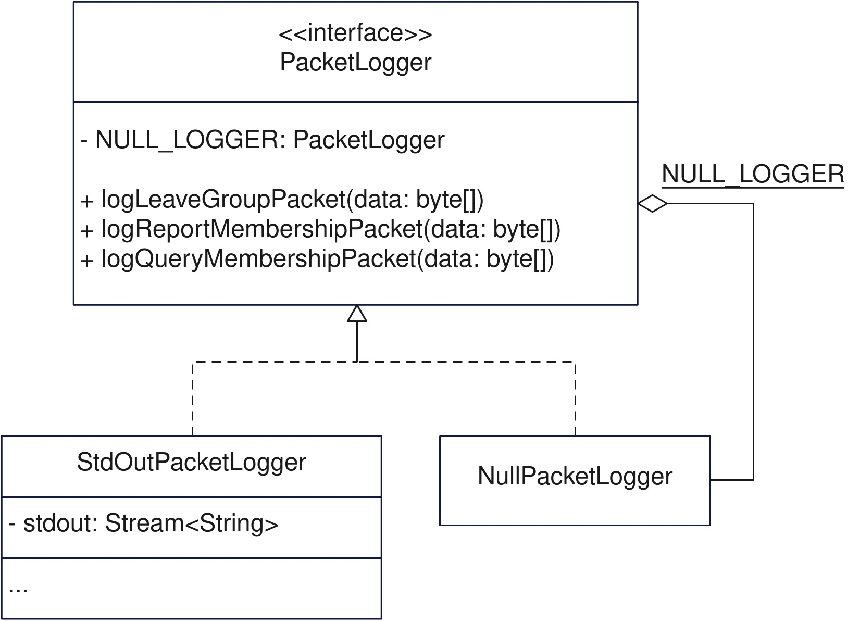
\includegraphics[width=0.66
    \textwidth]{def_null_logger}
    \caption{Default Values: Null logger}
    \label{fig:def_null_logger}
\end{figure}

\begin{figure}[!htb]
    \centering
    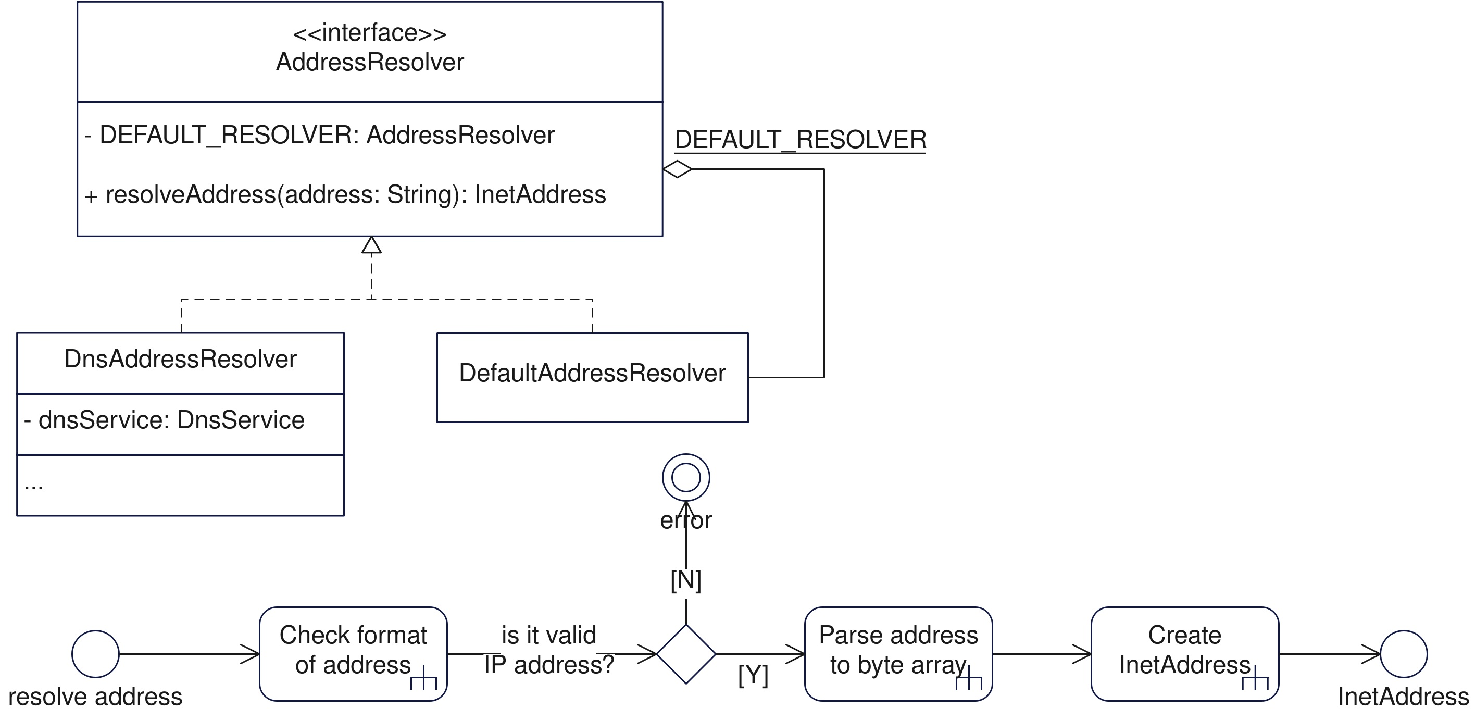
\includegraphics[width=1.0
    \textwidth]{def_default_address_resolver}
    \caption{Default Values: Default address resolver}
    \label{fig:def_default_address_resolver}
\end{figure}

Benefits of the Default Values approach:

\begin{itemize}
    \item Improved readability of the method signature - it is clear which parameters are optional and what values
    are used if these parameters are not specified by caller.
    Definition of the method itself is used as a documentation.
    \item Removed handling of null references or values in the implementation of the interface method
    (based on separation of concerns principle).
    It usually consists of repetitive conditional statements that check whether the parameter is null or not.
    Code is more readable and easier to maintain.
\end{itemize}

Drawbacks of the Default Values approach:

\begin{itemize}
    \item Limited flexibility - Default values are static and cannot be changed at runtime.
    This can limit the flexibility of your code, especially if you need to change these values based on certain
    conditions or configurations.
    \item For some complex types it is not always feasible to create a default implementation.
    If type defines method that returns value of some type, it is also necessary to mock return type.
    Also in some languages it is possible to mark a type or method as final, so it is not possible to create
    a subclass from it or override implementation of specific method.
    If type is defined in the external library, we cannot easily update its constraints.
\end{itemize}

Common use-cases of the Default Values approach:

\begin{itemize}
    \item Specification of default values for optional parameters that are not used frequently by clients
    deployed in production environment.
    These parameters can be used, for example, in the debugging mode or in the testing environment.
    \item Avoiding extensive overloading of the method signature - decreasing impact of API Rooting issue.
    If there are many optional parameters, it would be unpractical to create all possible combinations of methods.
    Additional interface methods increase maintenance cost.
\end{itemize}


\section{Parameter Object}
\label{sec:parameter_object}
Parameter Object is a design pattern that is used to group logically related method parameters into a separate entity
(usually data class or structure).
The method is then refactored to accept a single parameter object instead of multiple parameters.
The Parameter Object is usually immutable and contains only accessor methods.

Figure~\ref{fig:group_single_entity} demonstrates extraction of 3 parameters \textit{igmpType},
\textit{maxResponseTime} and \textit{groupAddress} into a new class named \textit{IgmpPacket}.
\textit{IgmpPacketWriter} service is then refactored to accept 2 parameters instead of 5 in the method
\textit{writeIgmpPacket}: \textit{igmpPacket} and \textit{outputStream}.
Class \textit{IgmpPacket} also contains Factory methods for simple creation of different types of IGMP packets.
These Factory methods are responsible for filling in correct constant values for each type of IGMP packet.

\begin{figure}[!htb]
    \centering
    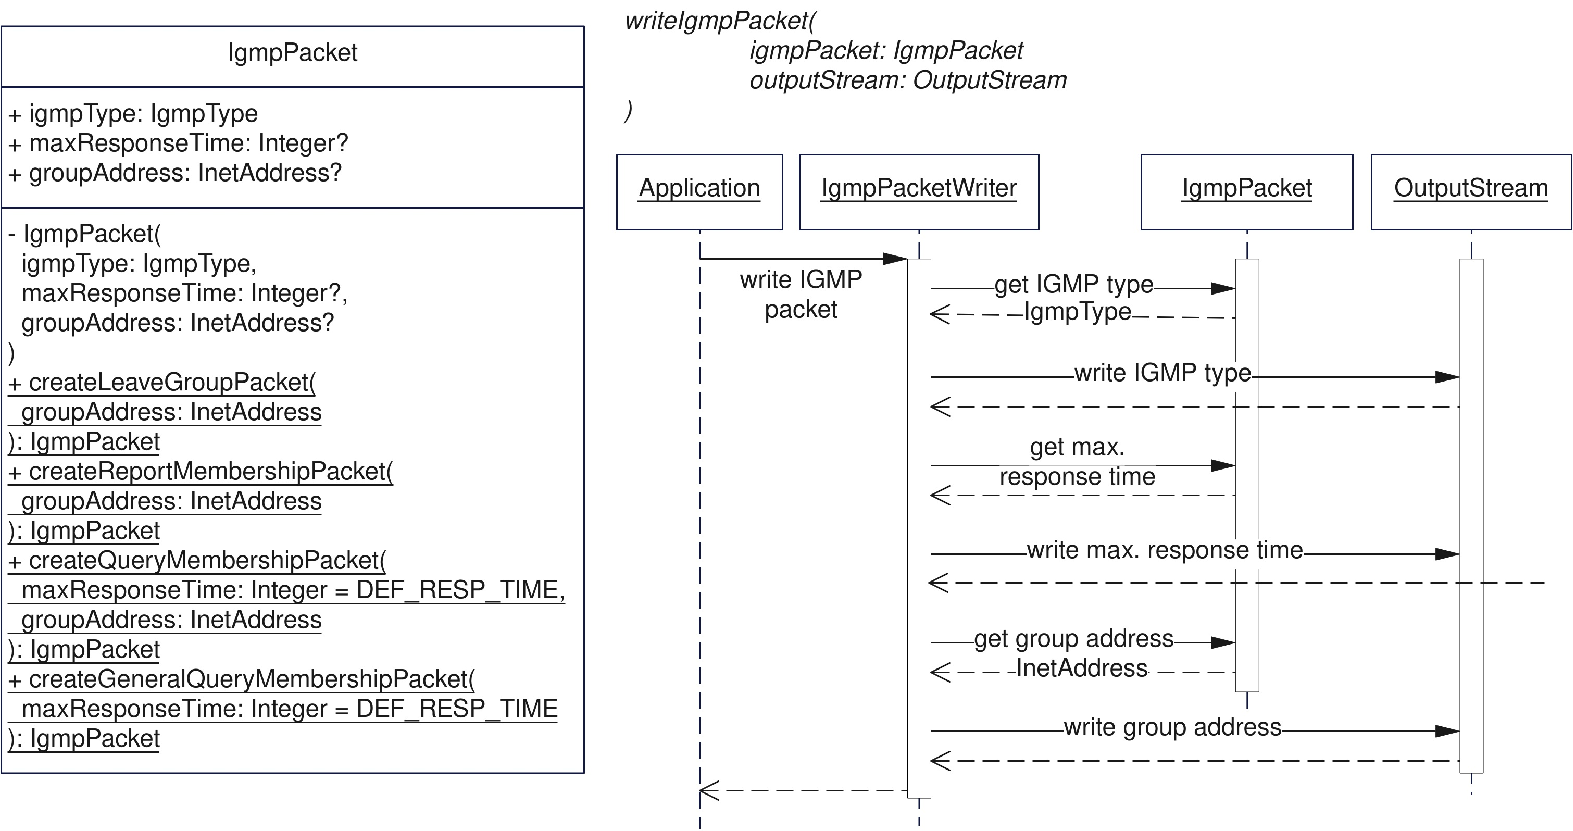
\includegraphics[width=1.0
    \textwidth]{group_single_entity}
    \caption{Parameter Objects: Extraction of a group of parameters into a separate class}
    \label{fig:group_single_entity}
\end{figure}

Instead of using Factory methods, it is possible to use Builder pattern to create
instances of \textit{IgmpPacket} class.
Builder pattern is more suitable if there are many optional parameters that can be set by client.
Figure~\ref{fig:group_build_single_entity} shows how Builder pattern can be used to create an instance
of \textit{IgmpPacket} class.
The whole building process happens in the \textit{build} method that is called by client after setting all necessary
parameters.
Building method usually contains logic around validation of parameters, setting default values, or transformation
of values into a different format.

\begin{figure}[!htb]
    \centering
    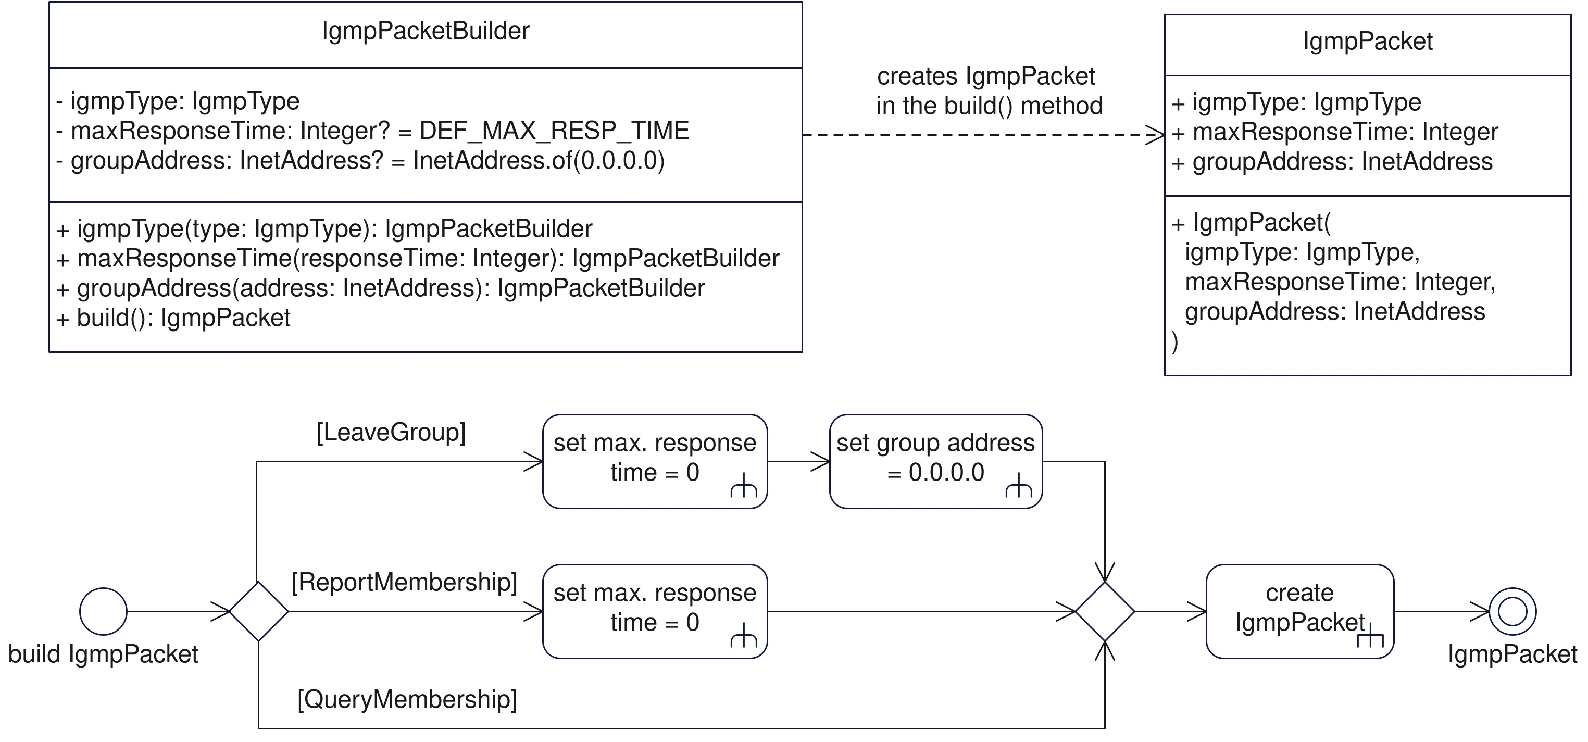
\includegraphics[width=1.0
    \textwidth]{group_build_single_entity}
    \caption{Parameter Objects: Using Builder pattern to create IgmpPacket object}
    \label{fig:group_build_single_entity}
\end{figure}

The following Figures~\ref{fig:group_build_structure} displays next iteration Builder design pattern on this example.
In this case, builder class creates specific instance of \textit{IgmpPacket} subtype - \textit{IgmpLeaveGroupPacket},
\textit{IgmpReportMembershipPacket}, or \textit{IgmpQueryMembershipPacket}.
Definition of multiple subtypes of \textit{IgmpPacket} class is better approach than relying on single entity
if there are multiple structural differences between IGMP packet types or if it is necessary to bound some behavior
to specific type of IGMP packet.
If there is some common behavior or fields that are shared between all IGMP packet types, it is additionally good
to move them to newly created template class that is placed between \textit{IgmpPacket} and its subtypes
in the inheritance structure.

\begin{figure}[!htb]
    \centering
    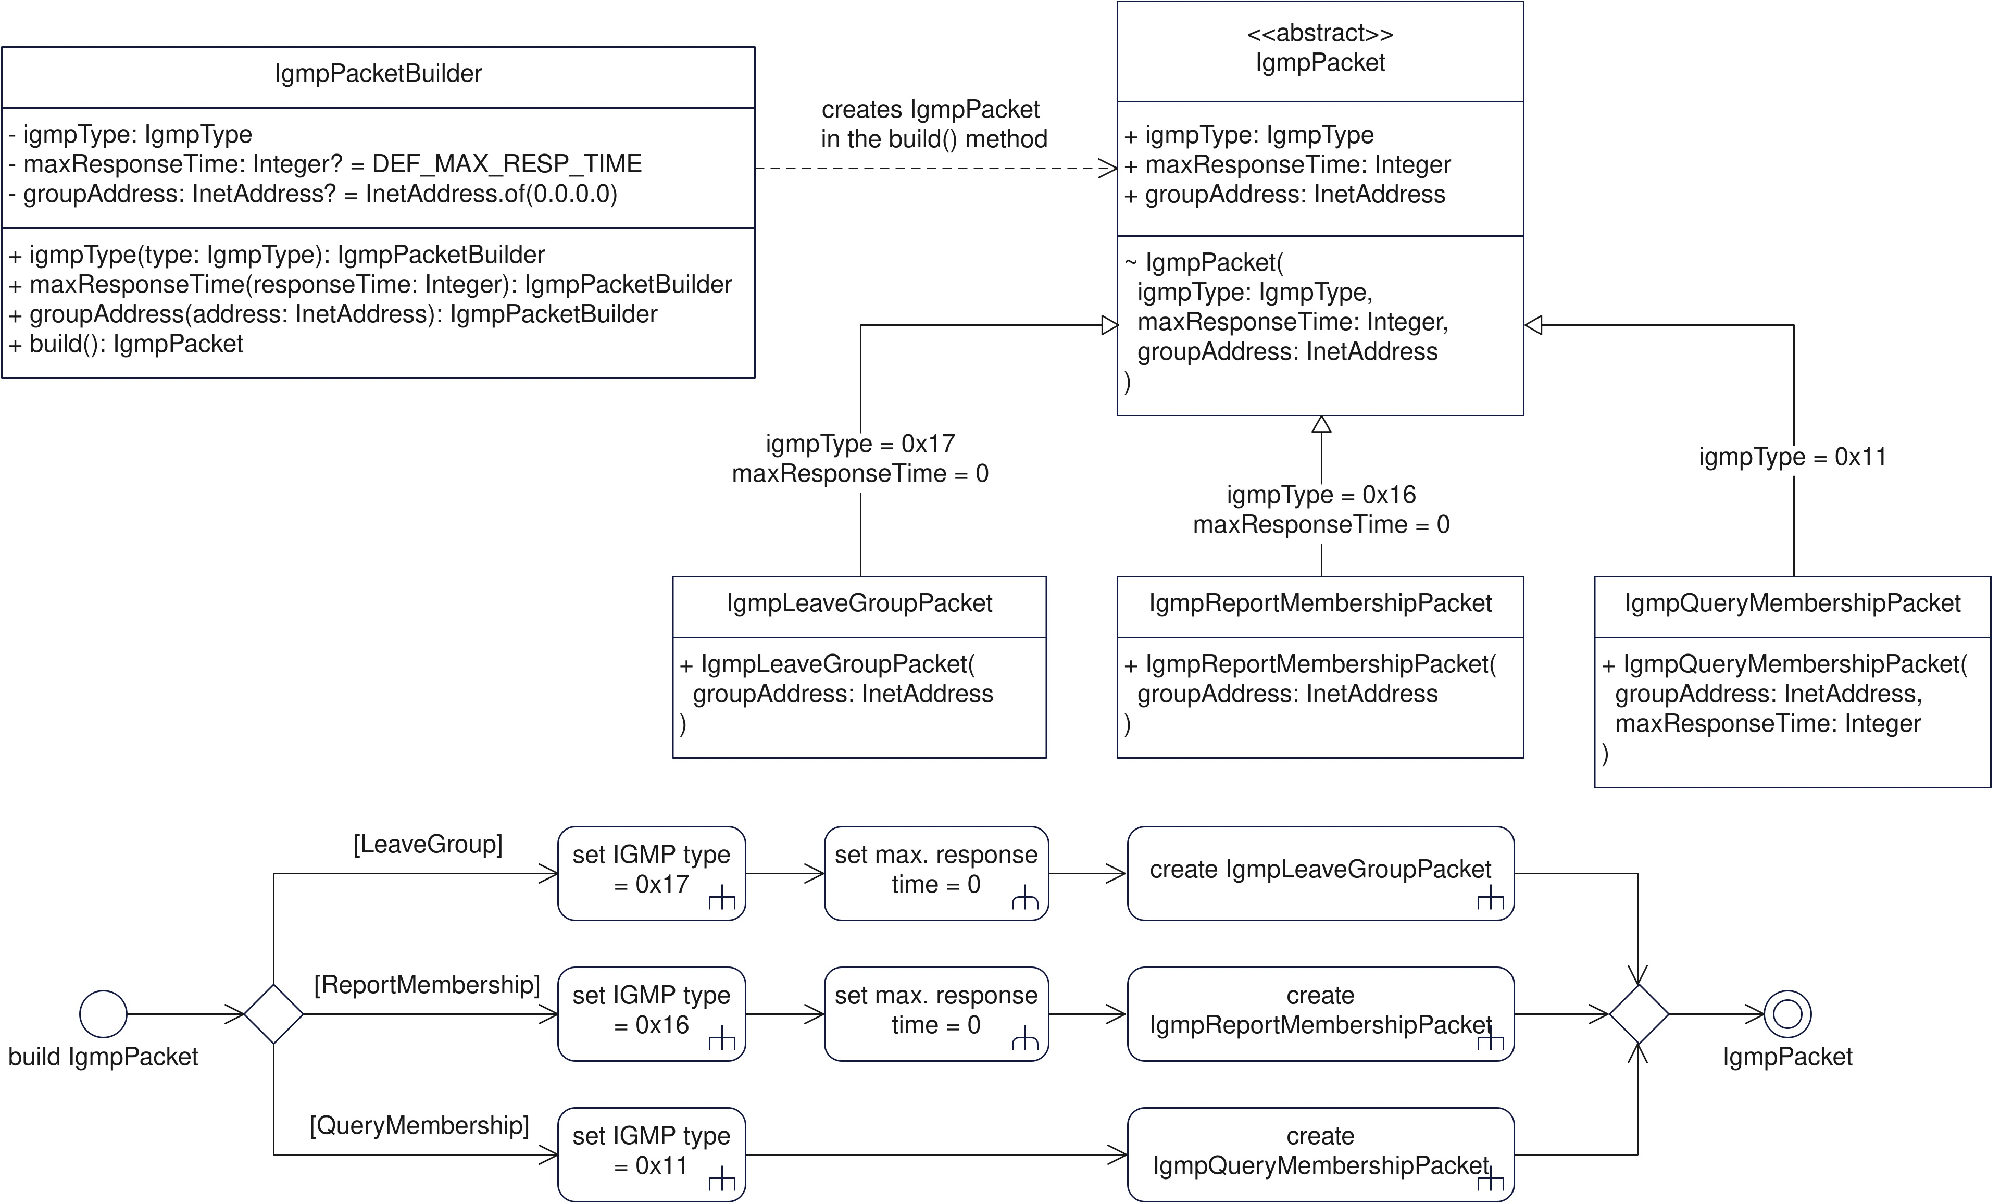
\includegraphics[width=1.0
    \textwidth]{group_build_structure}
    \caption{Parameter Object: Using Builder pattern to create object of IgmpPacket subtype}
    \label{fig:group_build_structure}
\end{figure}

Sometimes it is better to move responsibility for writing IGMP packet to output stream from \textit{IgmpPacketWriter}
to \textit{IgmpPacket} itself.
This is demonstrated in the Figure~\ref{fig:group_write_from_igmp_packet}.
The advantages of this approach is that it is possible to use polymorphism to invoke correct method for writing
IGMP packet to output stream and \textit{IgmpPacketWriter} does not have to access exposed fields
of \textit{IgmpPacket} class.
The disadvantage is that \textit{IgmpPacket} is now tightly coupled with \textit{OutputStream} and maybe
other serialization business logic.
Since \textit{IgmpPacket} is part of the public API such coupling between implementation and API can be problematic
in the future from the view of dependency management and code maintainability.

\begin{figure}[!htb]
    \centering
    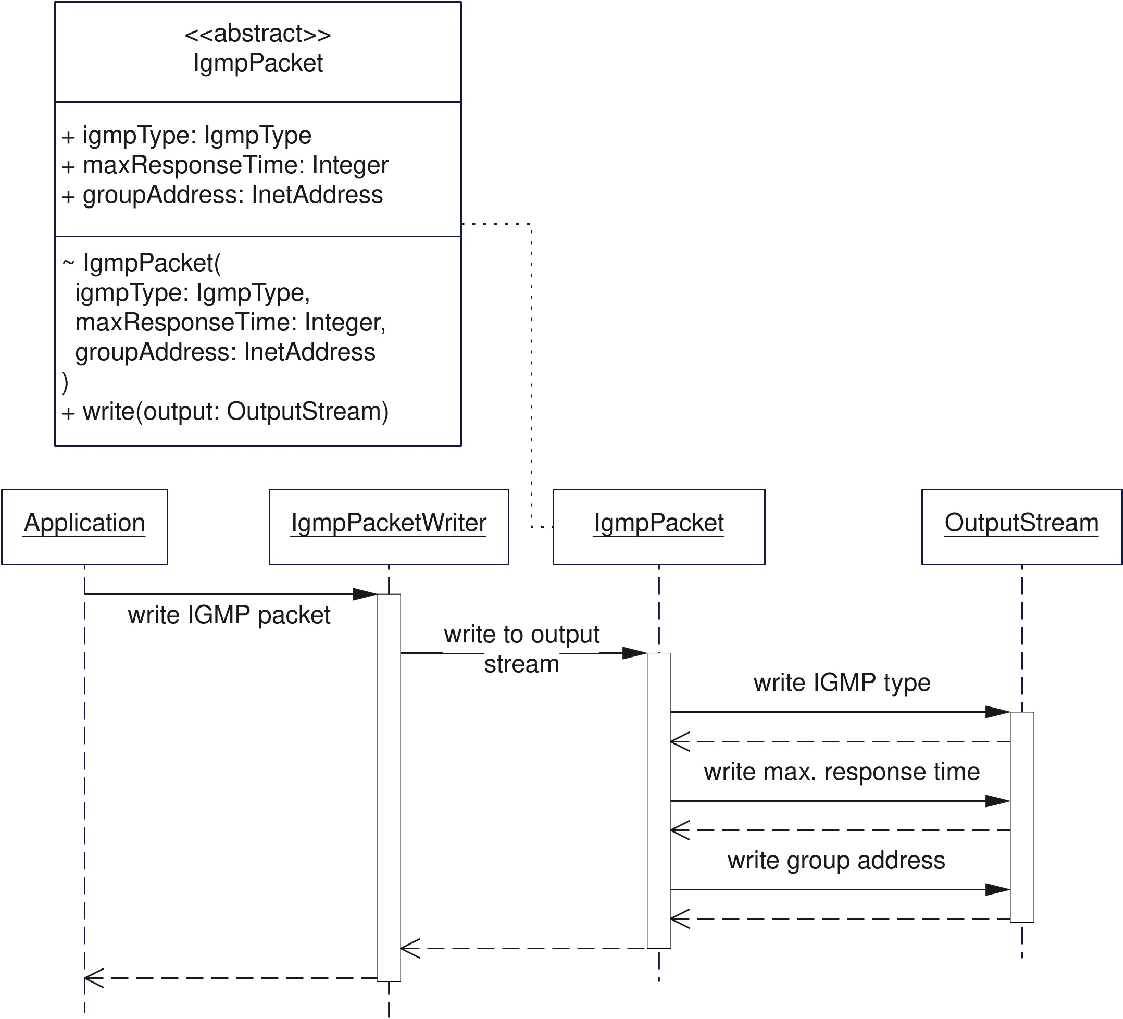
\includegraphics[width=0.8
    \textwidth]{group_write_from_igmp_packet}
    \caption{Parameter Object: Moving write responsibility from IgmpPacketWriter to IgmpPacket}
    \label{fig:group_write_from_igmp_packet}
\end{figure}

The last variation of Parameter Object approach is shown in the Figure~\ref{fig:group_visitor} with
applied Visitor design pattern.
In this scenario, \textit{IgmpPacket} class accepts \textit{IgmpPacketProcessor} as a parameter
in the method \textit{process}.
\textit{IgmpPacketProcessor} represents the interface and \textit{IgmpPacketWriter} implements this interface
- there is one method implementation for each subtype of \textit{IgmpPacket}.
The advantage of this approach in comparison with previous on Figure~\ref{fig:group_write_from_igmp_packet}
is that \textit{IgmpPacket} is not directly coupled with implementation logic.
Rather, there is another abstraction layer between \textit{IgmpPacket} and \textit{IgmpPacketWriter} in form
of generic visitor interface \textit{IgmpPacketProcessor}.
Disadvantage of this approach is the presence of double-dispatching mechanism and the additional implementation
complexity connected with it.

\begin{figure}[!htb]
    \centering
    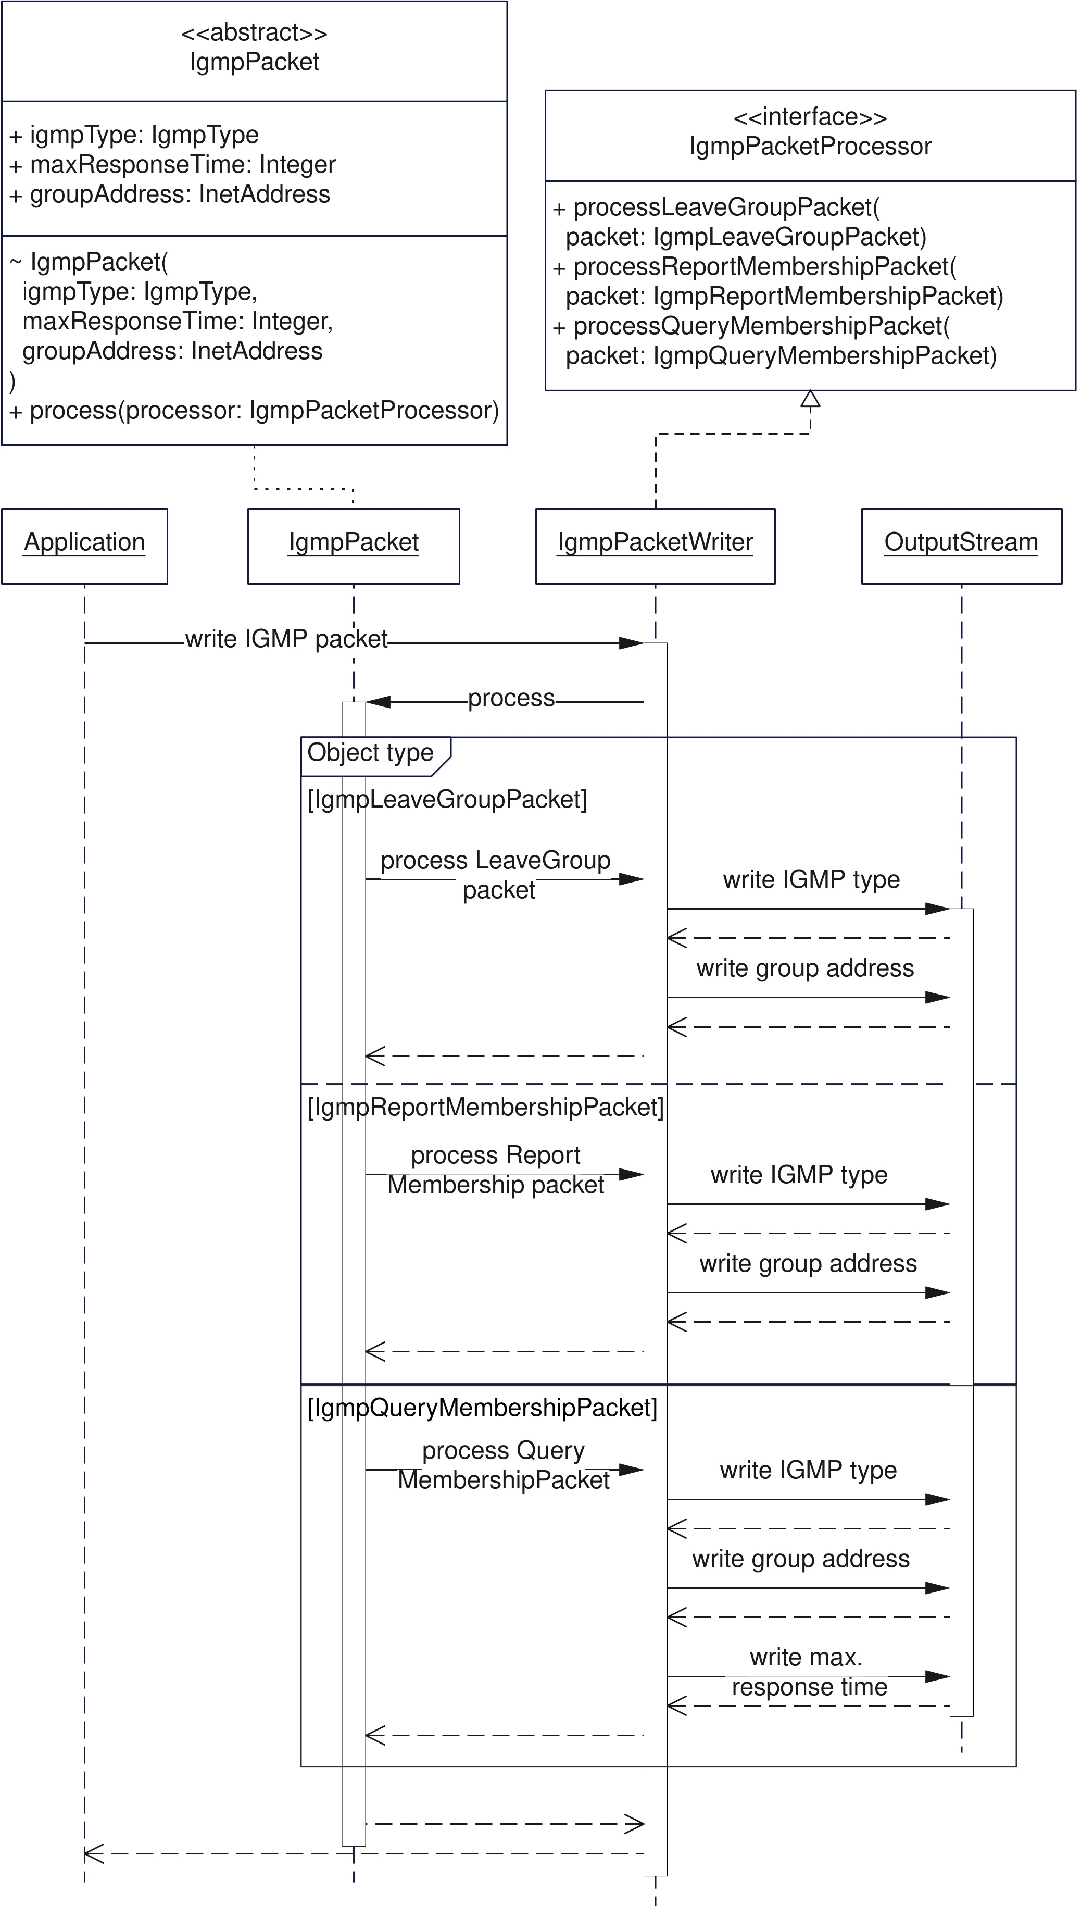
\includegraphics[width=0.75
    \textwidth]{group_visitor}
    \caption{Parameter Objects: Using Visitor design pattern to invoke actions on IgmpPacket subtype}
    \label{fig:group_visitor}
\end{figure}

Benefits of the Parameter Object design pattern:

\begin{itemize}
    \item Grouping of closely related parameters into a single entity improves readability of the code.
    It is also possible to create multiple Parameter Objects that are used in the same method.
    \item Parameter Object can be reused in multiple interface methods and also in the implementation of these methods.
    \item It makes API less fragile, if construction of Parameter Object is done by Builder or Factory pattern
    and not directly by calling constructor of the created class.
\end{itemize}

Drawbacks of the Parameter Object design pattern:

\begin{itemize}
    \item Risk of encapsulation violation if Parameter Object is mutable.
    \item Parameter Object can be overused, and it can lead to creation of too many classes.
    \item Higher risk of exposing implementation details though API that uses this design pattern.
\end{itemize}

Common use-cases of the Parameter Object design pattern:

\begin{itemize}
    \item Compressing long list of parameters into single or just few Parameter Objects.
    \item Grouping optional parameters into Parameter Object and this way avoid method overloading
    and existence of nullable parameters.
    \item Assuring consistency of method definitions by grouping the repetitive list of parameters
    into Parameter Object.
\end{itemize}


\section{API Strategies}
\label{sec:api_strategies}
API Strategies is based on creation of multiple subtypes of the service.
It uses Strategy design pattern to create a set of implementations that implement the same service definition\@.

The Figure~\ref{fig:strat_structure_and_behaviour} shows the example of the API Strategies.
The service \textit{IgmpPacketWriter} is decomposed into 3 subtypes: \textit{IgmpLeaveGroupWriter},
\textit{IgmpQueryMembershipWriter}, and \textit{IgmpReportMembershipWriter} - each of them implements
the \textit{writePacket} method in a different way.
The subtypes of \textit{IgmpPacketWriter} are also bound to corresponding subtypes of the \textit{IgmpPacket} class
using template parameter \textit{T} that must extend \textit{IgmpPacket} type.
Afterward, specific implementations of the service can work directly with the correct subtype of the packet.
Parts of the implementations that are common in all subtypes of service can be moved to additional abstract
class that realizes \textit{IgmpPacketWriter} interface (using Template design pattern).

\begin{figure}[!htb]
    \centering
    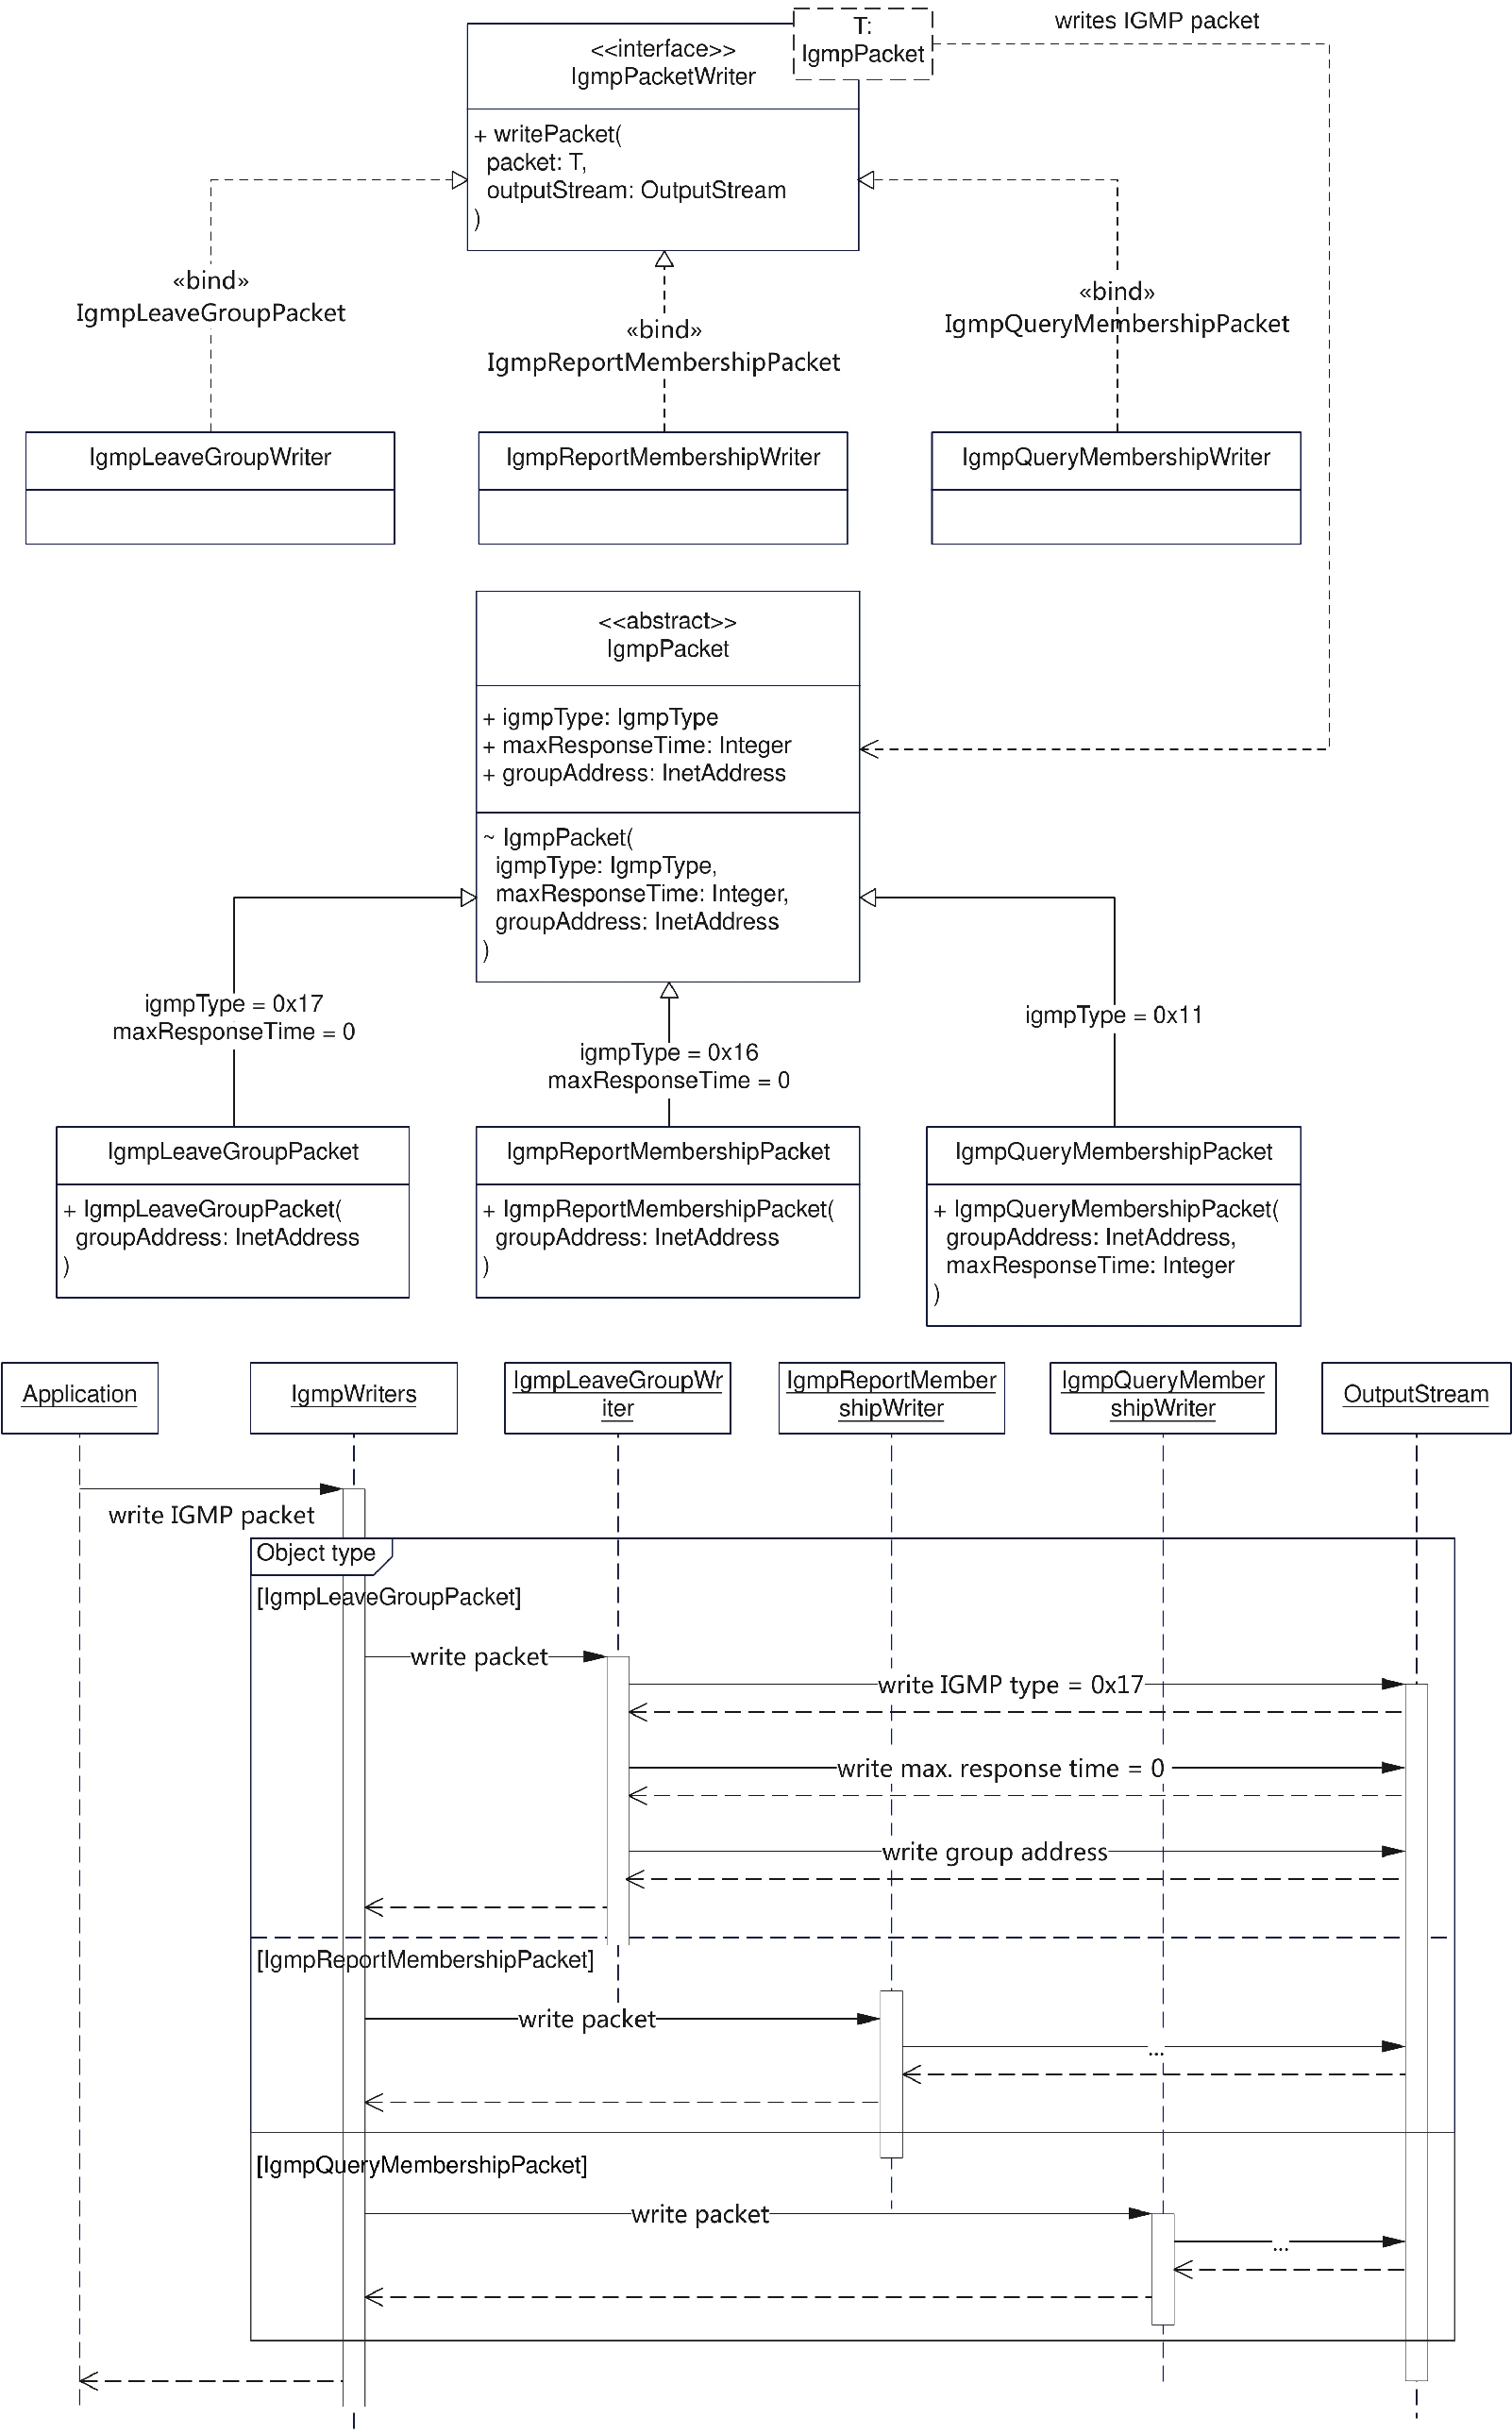
\includegraphics[width=0.85
    \textwidth]{strat_structure_and_behaviour}
    \caption{API Strategies: Decomposition of API into multiple subtypes}
    \label{fig:strat_structure_and_behaviour}
\end{figure}

Benefits of the API Strategies:

\begin{itemize}
    \item This approach can easily be combined with other methodologies that focus on design of interface
    method parameters.
    \item Extensibility of the API - It is possible to add new implementations of the service
    without altering existing implementations.
    \item Testing experimental implementations is much easier using this approach than by passing additional arguments
    to the interface methods or adding new interface methods.
\end{itemize}

Drawbacks of the API Strategies:

\begin{itemize}
    \item Service implementation usually contain also code related to the lifecycle of the service
    (e.g.\ initialization and destruction of the service).
    This lifecycle must be managed for all versions of the service.
    \item Multiple implementations of the service must be distinguished using another identifier.
    This problem is solved by Dependency Injection (DI) framework that supports assigning of the additional qualifier
    to the service implementation.
    \item Maintaining multiple implementations of the service can be difficult because of the code duplication
    between the implementations.
    Usually some parts of the implementation are common in all implementations and can be moved to the template class.
    However, the goal of the API Strategies is to create services implementations that are as isolated as possible.
    This can result in either code duplication or in the creation of additional abstraction layers that are difficult
    to maintain.
    Figure~\ref{fig:strat_infected_tree} shows an example of the more complex service inheritance tree.
\end{itemize}

\begin{figure}[!htb]
    \centering
    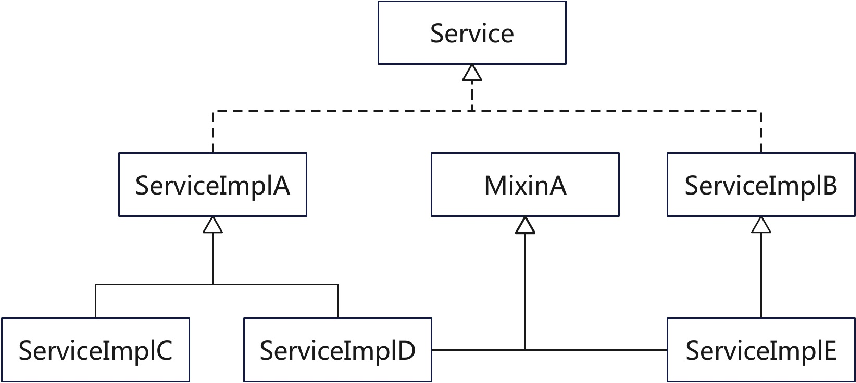
\includegraphics[width=0.66
    \textwidth]{strat_infected_tree}
    \caption{API Strategies: Example of the more complex service inheritance tree}
    \label{fig:strat_infected_tree}
\end{figure}

Common use-cases of the API Strategies:

\begin{itemize}
    \item Multiple implementations in different contexts are required.
    For example, there could be single generic service that defines writing of the packet to the network interface.
    However, there could be multiple types of the network interfaces (e.g.\ Ethernet, Wi-Fi, etc.), each of them
    requiring different strategy for writing the packet to the interface.
    \item There could be multiple implementations of the service that works in different environments.
    For example, the service that performs system calls must be implemented differently under different
    versions of the operating system if certain system calls are different.
    \item Creation of mocked implementations of the service for testing purposes (unit or integration tests).
\end{itemize}


\section{Model-Driven API}
\label{sec:model_driven_api}
In the Model-Driven API, in the first step the developer writes model of the operations, usually using the
specialized language used for this purpose.
Afterward there are 2 possible ways how the model can be used depending on the modeling language and technology stack:

\begin{enumerate}
    \item Through generation phase: The API generator is used for generation of the code of the API\@
    (entities that represent input and output structure of the modeled operations).
    To be able to consume and implement Model-Driven API, the developer must execute the generation phase.
    \item Directly by target technology: The API generator is not used and the model is directly parsed
    by the target technology compiler or interpreter.
    In this case model is usually more tightly coupled with the source code of the API implementation
    than in the previous case.
\end{enumerate}

The implementation of API is either written manually by the developer or in some simpler cases it can be generated
directly from the model.
For example, implementation of basic Create/Read/Update/Delete (CRUD) database or user-facing operations can usually
be generated directly from the model.

Benefits of the Model-Driven API:

\begin{itemize}
    \item Consistency of the API - The API is consistent by design, because it is generated from the model
    (for example, syntax and used design patterns).
    The design patterns and approaches that are described in this article are automatically applied.
    The API clients may also use the same model to generate or verify API calls.
    \item Documentation - The model can be used to generate documentation of the API\@.
    The whole process can be automated.
    \item Technology-agnostic - The model is usually technology-agnostic, so it can be used to generate API
    in various programming languages and technologies.
    \item Reduction of boilerplate code - The model can be used to generate API implementation including
    input/output entities, which reduces the amount of boilerplate code that the developer has to write.
    Some generators also support full or partial generation of queries and mutations.
    \item It is less error-prone than manual implementation - The model is usually validated by the generator
    before the code is generated.
    Additionally, the API itself is constrained by the model, which reduces the possibility of errors.
\end{itemize}

Drawbacks of the Model-Driven API:

\begin{itemize}
    \item Limited flexibility - The model is usually more constrained than the API implementation.
    It may not be possible to express all the features of the API in the model.
    \item Additional complexity - The model adds next layer of complexity.
    The developer has to learn the modeling language and use the API generator when the model changes.
    Because of this additional complexity, the Model-Driven API is usually not used in the internal API between
    components in the same service.
    It is more suitable for the external API connecting other services and clients.
    \item Dependency on the model and tools - The development process becomes heavily dependent on the modeling and
    generation tools.
    If these tools are not maintained or become obsolete, it could pose significant challenges.
\end{itemize}

Common use-cases of the Model-Driven API:

\begin{itemize}
    \item If service consists of multiple components that uses different technologies or programming languages,
    the Model-Driven API can be used to generate API for each component in the target technology.
    \item Model-Driven API is handy for generation of the repetitive code (for example, CRUD operations)
    to reduce the amount of boilerplate code and assure consistency.
    For example, if there is complex data-tree, and you need to implement CRUD operations for each node in the tree,
    it would be very tedious to write all the API and its implementation manually.
\end{itemize}


\section{Summary}
\label{sec:summary}
Figure~\ref{fig:metamodel} summarizes all presented approaches with design patterns and the relations between them.

\begin{figure}[!htb]
    \centering
    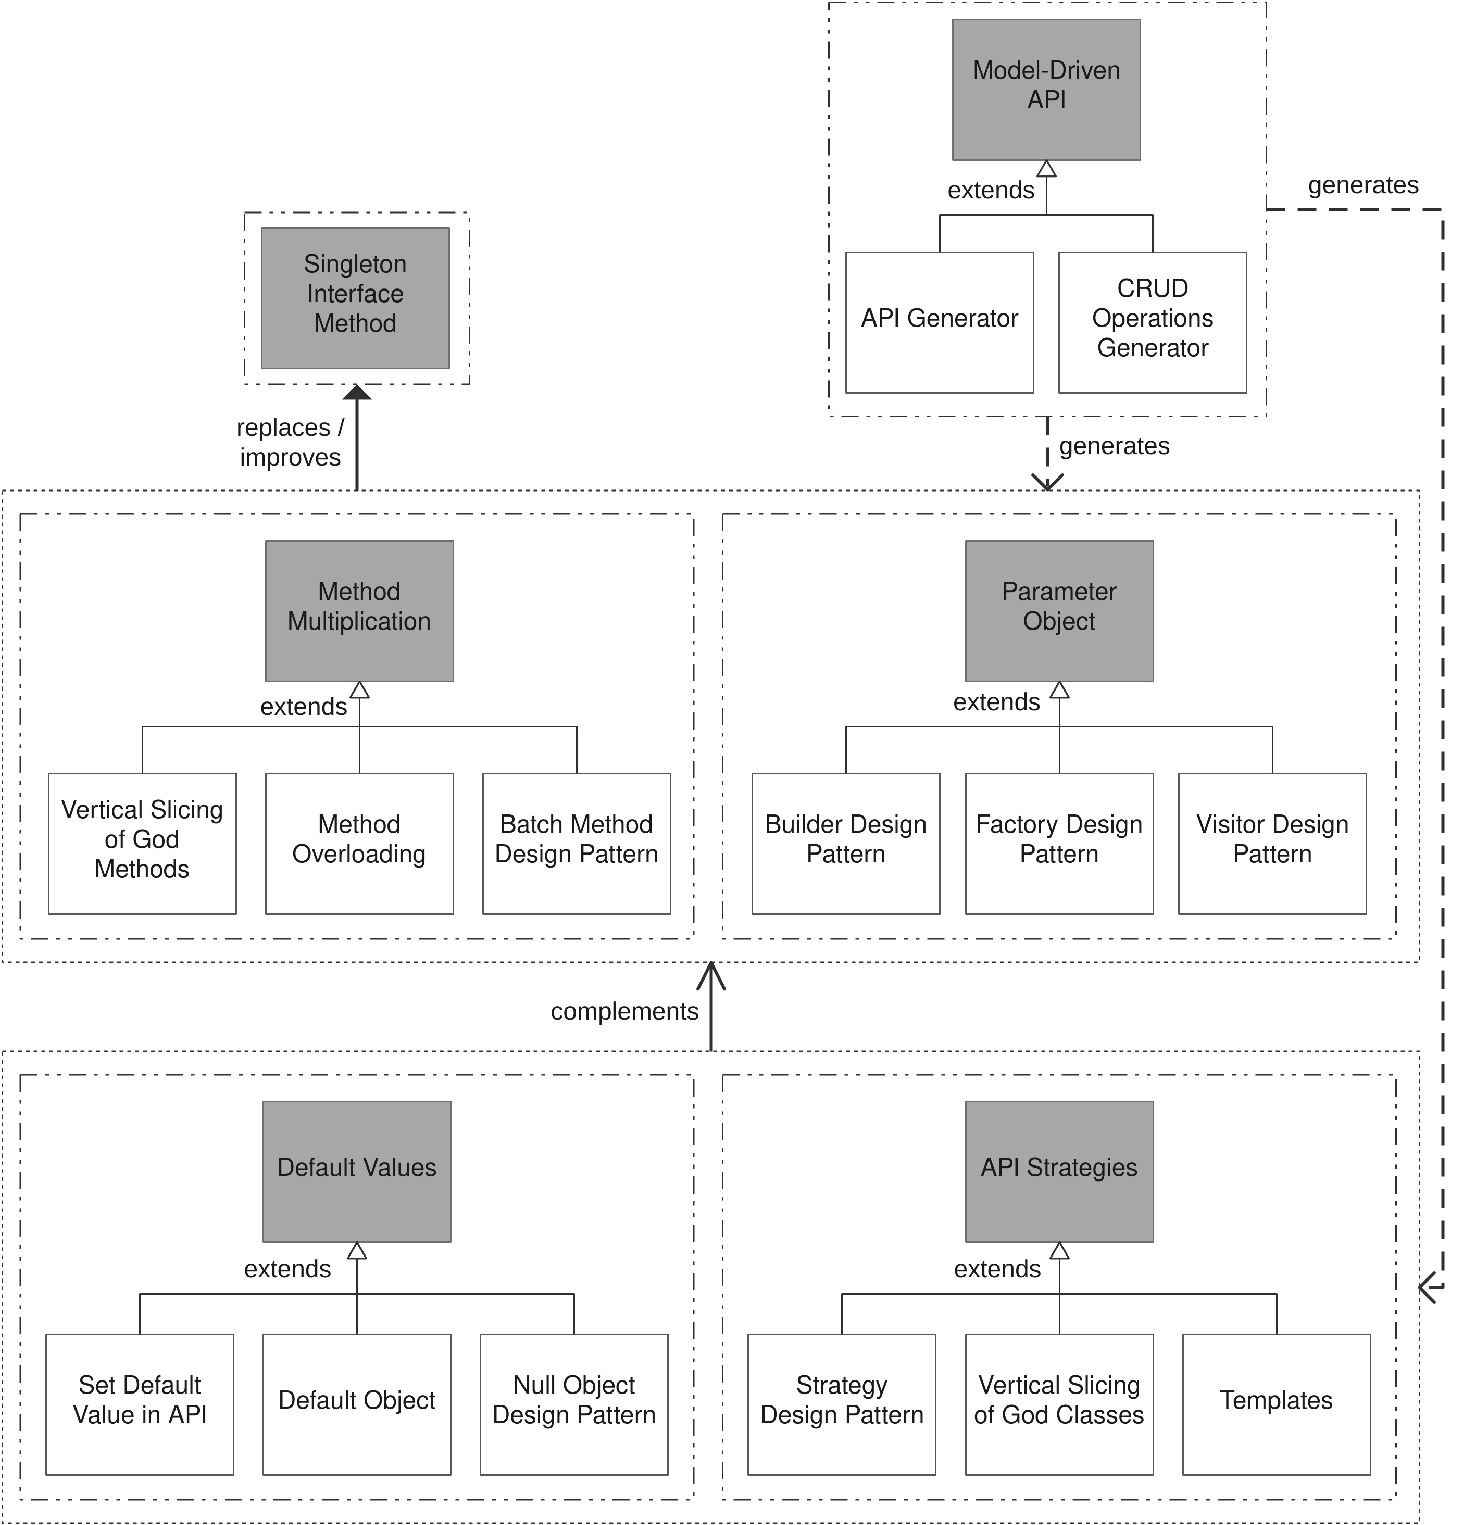
\includegraphics[width=1.0
    \textwidth]{metamodel}
    \caption{Summary: Metamodel containing overview of presented approaches and patterns}
    \label{fig:metamodel}
\end{figure}

The guide starts with the Singleton Interface Method, which is the most basic approach for modeling internal
synchronous APIs.
This modeling approach is suitable for simple methods without the need for flexibility and extensibility.
However, there are many cases when this approach is not suitable, and more advanced design patterns are required
to preserve code quality.

The Method Multiplication focuses on the vertical slicing of interface methods into more granular interface methods,
thus breaking God Methods that usually occur in Singleton Interface Methods.
On the other side, the Default Values approach does not try to break methods into smaller pieces but rather aims
to reduce the number of methods by providing default values for optional parameters.
From the view of the metamodel, both Method Multiplication and Default Values are successors
of the Singleton Interface Method when dealing with a more complex API with more responsibilities
or expectations for API evolution.

The Parameter Object represents the next design pattern that can be used for the simplification of method signatures
and reusability of a group of parameters.
There are multiple ways to construct a Parameter Object, for example, using Builder or Factory design patterns.
It is also possible to construct more complex Parameter Objects by aggregating other objects
or introducing inheritance between different types of Parameter Objects.

The API Strategies approach goes beyond Method Multiplication and extends the vertical slicing of interface methods
by introducing different API subtypes.
This is handy if there is a need to provide a similar API for different data types or in different contexts.
Parameter Object and API Strategies are most often used as the next step in the design or refactoring process
after Method Multiplication or Default Values are applied but still not enough to achieve
the desired decomposition level.
All of these approaches and design patterns are not mutually exclusive and can be used together.

The final section presents the concept of Model-Driven API, which is based on the idea of defining the model
and generating API interfaces and entities from the model.
The generation of API ensures consistency and reduces the amount of boilerplate code.
However, it also introduces additional complexity and dependency on the model and tools.
Because of this, it is usually used for external APIs connecting different services and clients.


\newpage
\bibliographystyle{ieeetr}
\bibliography{references}

\end{document}
